\documentclass[11pt,a4paper,openany]{book}

\usepackage{fontspec}
\setmainfont{Times New Roman}
\setsansfont{Arial}
\setmonofont{Menlo}
\usepackage[a4paper,inner=2.7cm,outer=2.2cm,top=2.45cm,bottom=2.65cm,headheight=16pt]{geometry}
\usepackage{amsmath,amssymb,mathtools,bm}
\usepackage{graphicx,booktabs,longtable,tabularx,array}
\graphicspath{{assets/}}
\usepackage{xcolor,tcolorbox,enumitem,titlesec,fancyhdr,caption,microtype}
\tcbuselibrary{skins,breakable}
\usepackage[colorlinks=true,linkcolor=blue!45!black,urlcolor=blue!45!black,citecolor=blue!45!black]{hyperref}
\numberwithin{equation}{chapter}
\numberwithin{figure}{chapter}
\numberwithin{table}{chapter}
\setcounter{tocdepth}{1}
\setcounter{secnumdepth}{2}
\setlength{\parindent}{1.5em}
\setlength{\parskip}{0.25em}
\setlength{\emergencystretch}{2em}

\definecolor{navy}{HTML}{1F4E79}
\definecolor{teal}{HTML}{1E6E5B}
\definecolor{brick}{HTML}{B33A3A}
\definecolor{papergray}{HTML}{F3F5F6}

\titleformat{\part}[display]{\centering\sffamily\bfseries\color{navy}}{PART \Roman{part}}{1em}{\Huge}
\titleformat{\chapter}[display]{\sffamily\bfseries}{\color{navy}\Large CHAPTER \thechapter}{0.5em}{\Huge}[\vspace{0.5em}\color{navy}\titlerule]
\titleformat{\section}{\Large\sffamily\bfseries\color{navy}}{\thesection}{0.7em}{}
\titleformat{\subsection}{\large\sffamily\bfseries}{\thesubsection}{0.7em}{}
\pagestyle{fancy}
\fancyhf{}
\fancyhead[LE]{\small\color{navy}\thepage\qquad\nouppercase{\leftmark}}
\fancyhead[RO]{\small\color{navy}\nouppercase{\rightmark}\qquad\thepage}
\renewcommand{\headrulewidth}{0.4pt}
\fancypagestyle{plain}{\fancyhf{}\fancyfoot[C]{\color{navy}\thepage}\renewcommand{\headrulewidth}{0pt}}
\captionsetup{font=small,labelfont={bf,color=navy},justification=justified,singlelinecheck=false}

\tcbset{
  keybox/.style={breakable,colback=navy!5,colframe=navy!65,boxrule=0.7pt,arc=2pt},
  resultbox/.style={breakable,colback=teal!5,colframe=teal!70,boxrule=0.7pt,arc=2pt},
  cautionbox/.style={breakable,colback=brick!5,colframe=brick!65,boxrule=0.7pt,arc=2pt}
}
\newcommand{\chapterguide}[1]{\begin{tcolorbox}[keybox,title=Chapter guide]#1\end{tcolorbox}}
\newcommand{\chapterend}[1]{\section*{Chapter summary}\addcontentsline{toc}{section}{Chapter summary}\begin{tcolorbox}[resultbox]#1\end{tcolorbox}\subsection*{Questions for reflection}\begin{enumerate}[leftmargin=1.7em]\item Reconstruct the main argument without looking at the final criterion. Which assumptions are essential?\item Design one numerical check that could falsify the conclusion rather than merely illustrate it.\end{enumerate}\clearpage}
\newcommand{\dd}{\,\mathrm{d}}
\newcommand{\Rea}{\operatorname{Re}}
\newcommand{\Ima}{\operatorname{Im}}

\hypersetup{
 pdftitle={Traffic-Flow Stability: Microscopic Models, Macroscopic Continuum Theory, Experiments, and Control},
 pdfauthor={Changxin Wan},
 pdfsubject={Traffic-flow stability, numerical experiments, continuum models, and control applications},
 pdfkeywords={traffic stability, IDM, string stability, LWR, PW, ARZ, nonlinear waves, AV control}
}

\begin{document}
\frontmatter
\begin{titlepage}
\centering
\vspace*{3.2cm}
{\sffamily\bfseries\color{navy}\fontsize{29}{34}\selectfont Traffic-Flow Stability\par}
\vspace{0.6cm}
{\sffamily\Large Microscopic Models, Macroscopic Continuum Theory,\par Numerical Experiments, and Control\par}
\vspace{2cm}
{\Large Changxin Wan\par}
\vfill
{\large Expanded English draft (not the final parallel translation)\par}
{\small August 2026\par}
\end{titlepage}

\chapter*{Preface to the English Edition}
\addcontentsline{toc}{chapter}{Preface to the English Edition}
Traffic congestion is not only a question of demand exceeding capacity. Even when the average demand is held constant, a small speed fluctuation may decay, persist, or amplify into stop-and-go traffic. Stability analysis provides a language for deciding which of these outcomes is expected and for designing vehicles or traffic controls that change the outcome \cite{treiber2013,wilson2011}.

This expanded English draft is a working companion to the Chinese book and online laboratory. It follows the analytical route of car-following dynamics, local and string stability, heterogeneous and connected vehicles, weakly nonlinear waves, continuum traffic models, microscopic--macroscopic consistency, trajectory-data evidence, and control applications. It retains worked numerical examples, experimental protocols, figure interpretation, questions for reflection, and appendices of stability criteria and reproducibility guidance. A chapter-by-chapter unabridged translation is maintained separately as the next editorial target; this draft must not be cited as a page-for-page replacement for the Chinese edition.

The browser laboratory is bilingual. Every experiment should be read in four layers: the equilibrium state, the analytical prediction, the imposed perturbation, and the measured response. A colored trajectory diagram alone is not a stability proof; it becomes evidence only when the working point, perturbation, numerical resolution, and quantitative metric are stated.

\tableofcontents

\mainmatter
\part{Microscopic Foundations}

\chapter{Car-Following Models: From Stimulus--Response to IDM}
\chapterguide{This chapter introduces the state variables and modeling assumptions needed before stability can be discussed. It also explains how a ring-road simulation is advanced in time.}

\section{What a car-following law describes}
Let vehicle $n-1$ be the leader of vehicle $n$. With position $x_n$, speed $v_n=\dot x_n$, vehicle length $\ell$, net gap
\begin{equation}
s_n=x_{n-1}-x_n-\ell,
\end{equation}
and approach rate $\Delta v_n=v_n-v_{n-1}$, a broad model class is
\begin{equation}
\dot v_n=F(s_n,v_n,\Delta v_n).
\end{equation}
The gap is a state, not an external parameter, because
\begin{equation}
\dot s_n=v_{n-1}-v_n=-\Delta v_n.
\end{equation}
On a ring of length $L$, indices are periodic and $x_0$ is interpreted as $x_N+L$. On an open road, the first vehicle instead requires a prescribed trajectory or a boundary controller. This distinction changes the admissible spatial modes and the meaning of disturbance amplification.

\section{GM, OVM, FVDM, and IDM}
The early Gazis--Herman--Rothery family formalizes a stimulus--response idea,
\begin{equation}
\dot v_n(t+\tau)=\alpha\frac{v_n(t)^m}{s_n(t)^l}\bigl[v_{n-1}(t)-v_n(t)\bigr].
\end{equation}
The optimal-velocity model separates relaxation toward a desired speed from the current gap,
\begin{equation}
\dot v_n=a\bigl[V(s_n)-v_n\bigr],
\end{equation}
and the full velocity-difference model adds relative-speed damping. The Intelligent Driver Model (IDM) combines free acceleration and collision-avoidance interaction:
\begin{align}
\dot v_n&=a\left[1-\left(\frac{v_n}{v_0}\right)^\delta-\left(\frac{s^*(v_n,\Delta v_n)}{s_n}\right)^2\right],\\
s^*(v,\Delta v)&=s_0+vT+\frac{v\Delta v}{2\sqrt{ab}}.
\end{align}
Here $v_0$ is desired speed, $T$ desired time gap, $s_0$ jam clearance, and $a,b$ the characteristic acceleration and comfortable deceleration. IDM is continuous, collision-averse under its intended operating assumptions, and has a physically interpretable equilibrium fundamental diagram.

\section{A ring-road RK4 update}
For state $y=(x_1,\ldots,x_N,v_1,\ldots,v_N)^\top$ and derivative $\dot y=f(y)$, classical RK4 uses
\begin{align}
k_1&=f(y^m),&k_2&=f(y^m+\tfrac12\Delta t k_1),\\
k_3&=f(y^m+\tfrac12\Delta t k_2),&k_4&=f(y^m+\Delta t k_3),\\
y^{m+1}&=y^m+\frac{\Delta t}{6}(k_1+2k_2+2k_3+k_4).
\end{align}
Every stage must recompute wrapped gaps and accelerations. Reusing the first-stage gap in later stages is not RK4 and can move the measured stability boundary.

For a three-vehicle ring, compute $s_1=x_3+L-x_1-\ell$, $s_2=x_1-x_2-\ell$, and $s_3=x_2-x_3-\ell$ after ordering positions consistently. A convergence check repeats the case with $\Delta t/2$ and compares growth rate, wave speed, and minimum gap.

\section{Open platoons, rings, and the data recorded by a simulation}
An open platoon has an externally prescribed leader. It is consequently the natural setting for a sinusoidal leader input, a vehicle-to-vehicle transfer ratio, and a recovery-time measurement. A ring has no leader and admits only the discrete spatial wavenumbers $k_m=2\pi m/N$. It is consequently the natural setting for a modal eigenvalue calculation and for observing self-excited stop-and-go waves. When vehicles are homogeneous, interactions are unidirectional, and $N$ is large, the two viewpoints approach one another. With bilateral interaction, nonlocal communication, delay, or heterogeneous ordering, they answer different questions and must not be interchanged.

For every numerical run the saved data should include unwrapped positions $x_n(t)$, display positions $x_n(t)\bmod L$, speeds, net gaps, accelerations, model parameters, the perturbation, and the integration step. A position--time trajectory diagram is then formed by plotting every sampled trajectory in the $(t,x)$ plane and coloring it by speed. A speed or gap space--time diagram samples the vehicle field onto a fixed vehicle-index or road-position grid. A probe plot is not a plot of every vehicle: it is the time history of a declared vehicle index, so that the reader can link a macroscopic colored band to a driver's experienced speed and clearance.

\section{Worked example W01: two RK4 steps for three IDM vehicles}
Take three identical IDM vehicles with $L=75$ m, $\ell=5$ m, and $\Delta t=0.2$ s. Let the initial state be
\begin{equation}
\bm x^0=(0,25,50)\ \mathrm m,\qquad
\bm v^0=(10.0,9.5,10.5)\ \mathrm{m/s}.
\end{equation}
All initial net gaps are 20 m; the third gap is $0+75-50-5$, which is where the periodic boundary is used. With the baseline IDM parameters, the first RK4 derivative is
\begin{equation}
K_1^x=(10.0000,9.5000,10.5000),\qquad
K_1^v=(0.085445,0.610732,0.000756).
\end{equation}
The common second-stage state is
\begin{equation}
\bm x_{(2)}=(1.0000,25.9500,51.0500),\quad
\bm v_{(2)}=(10.008545,9.561073,10.500076).
\end{equation}
Recomputing all three gaps and accelerations at each stage gives
\begin{center}
\small
\begin{tabular}{c c c}
\toprule
stage & $(s_1,s_2,s_3)$ [m] & $K_r^v$ [m/s$^2$]\\
\midrule
$K_1$ & $(20.000000,20.000000,20.000000)$ & $(0.085445,0.610732,0.000756)$\\
$K_2$ & $(19.950000,20.100000,19.950000)$ & $(0.099911,0.595463,-0.000597)$\\
$K_3$ & $(19.955253,20.093900,19.950847)$ & $(0.098995,0.595674,0.000187)$\\
$K_4$ & $(19.909911,20.188079,19.902010)$ & $(0.112605,0.580323,-0.000526)$\\
\bottomrule
\end{tabular}
\end{center}
Thus the first complete update is
\begin{align}
\bm x^1&=(2.001896,26.912012,52.100002)\ \mathrm m,\\
\bm v^1&=(10.019862,9.619111,10.499980)\ \mathrm{m/s},
\end{align}
and repeating the same four-stage calculation gives
\begin{equation}
\bm x^2=(4.008283,28.847237,54.199994)\ \mathrm m,\qquad
\bm v^2=(10.044800,9.732109,10.499983)\ \mathrm{m/s}.
\end{equation}
This example is not a stability test. Its purpose is to make the simultaneous state update explicit: updating vehicle 1 before computing vehicle 3 would insert vehicle order into the physics and create an unreported numerical coupling.

\chapterend{Microscopic stability begins with a closed dynamical system. Gap evolution, boundary conditions, and numerical-stage consistency are as important as the acceleration formula.}

\chapter{Equilibrium, Linearization, and Three Notions of Stability}
\chapterguide{We derive the generic linear model and distinguish local, string, and ring stability.}

\section{Uniform equilibrium}
At equilibrium $s_n=s_e$, $v_n=v_e$, and $\Delta v_n=0$, so
\begin{equation}
F(s_e,v_e,0)=0.
\end{equation}
For IDM this becomes
\begin{equation}
1-\left(\frac{v_e}{v_0}\right)^\delta-\left(\frac{s_0+v_eT}{s_e}\right)^2=0.
\end{equation}
On a ring, $s_e=L/N-\ell$. Perturbations $\delta s_n=s_n-s_e$ and $\delta v_n=v_n-v_e$ give, to first order,
\begin{align}
\delta\dot s_n&=\delta v_{n-1}-\delta v_n,\\
\delta\dot v_n&=f_s\delta s_n+f_v\delta v_n+f_{\Delta v}(\delta v_n-\delta v_{n-1}),
\end{align}
where the partial derivatives of $F$ are evaluated at equilibrium.

\section{Why differentiating the equilibrium identity is useful}
If the equilibrium speed is written $v_e=V(s_e)$, differentiate $F(s_e,V(s_e),0)=0$ with respect to $s_e$. The chain rule gives
\begin{equation}
f_s+f_vV'(s_e)=0,
\qquad V'(s_e)=-\frac{f_s}{f_v},
\end{equation}
provided $f_v\ne0$. The third argument remains zero along the equilibrium curve, hence its derivative contributes nothing. This identity connects the static equilibrium curve to dynamic partial derivatives but does not determine stability by itself.

\section{Three questions that must not be confused}
Local stability asks whether one follower returns after its leader is held at equilibrium. String stability asks whether a disturbance is amplified from one vehicle to the next on an open chain. Ring stability asks whether any spatial Fourier mode grows under periodic closure. A locally stable vehicle may still amplify disturbances along a platoon.

\section{The linearized state equation}
The preceding first-order equations can be written in a form that exposes the information path. Define
\begin{equation}
f_s=\left.\frac{\partial F}{\partial s}\right|_e,\qquad
f_v=\left.\frac{\partial F}{\partial v}\right|_e,\qquad
f_{\Delta v}=\left.\frac{\partial F}{\partial \Delta v}\right|_e.
\end{equation}
Then the perturbation acceleration is a restoring-gap term, an own-speed term, and a relative-speed term. In physically conventional car following, $f_s>0$: an increase in gap encourages acceleration. Usually $f_v<0$: an increase in own speed reduces acceleration. Usually $f_{\Delta v}<0$: approaching a slower leader reduces acceleration. These signs are informative but are not themselves a string-stability criterion because they do not specify how the three mechanisms balance over space and time.

The equilibrium derivative identity can also be obtained geometrically. The set $F(s,v,0)=0$ is a curve in the $(s,v)$ plane. Moving along it by $\dd s$ requires a speed change $\dd v=V'(s)\dd s$. Its tangent must satisfy $f_s\dd s+f_v\dd v=0$, which is exactly $V'=-f_s/f_v$. This is why the equilibrium fundamental diagram supplies wave-speed information even though it does not by itself determine the dynamic damping.

\section{Perturbation conventions and margins}
Throughout the book, a stability margin is the signed distance from a named analytical boundary. A positive long-wave margin means that the $k^2$ coefficient has the damping sign under the convention used in that chapter; a negative margin means that sufficiently long nonzero waves grow. A margin is not a collision certificate, a guarantee for finite disturbances, or a measure of comfort. It is a local, model-based quantity that must be checked by nonlinear simulation when a control is selected near the boundary.

\chapterend{Linearization turns a nonlinear model into a derivative-based local description. The same derivatives enter different criteria because local recovery, open-chain propagation, and periodic-mode growth are different experiments.}

\chapter{Local Stability and the Meaning of Two Roots}
\chapterguide{This chapter derives the second-order local equation, explains its two roots, and connects damping type to a numerical pulse experiment.}

Hold the leader speed fixed, so $\delta v_{n-1}=0$. Since $\delta\dot s=-\delta v$, differentiating once gives $\delta\ddot s=-\delta\dot v$. Substitution yields
\begin{equation}
\delta\ddot s-f_v\delta\dot s+f_s\delta s=0.
\end{equation}
Trying $\delta s=Ae^{\lambda t}$ gives
\begin{equation}
\lambda^2-f_v\lambda+f_s=0.
\end{equation}
The real-coefficient Routh--Hurwitz criterion for $\lambda^2+a_1\lambda+a_0$ requires $a_1>0$ and $a_0>0$. Thus
\begin{equation}
f_v<0,\qquad f_s>0.
\end{equation}

\section{Which root is observed?}
With distinct roots $\lambda_1,\lambda_2$,
\begin{equation}
\delta s(t)=C_1e^{\lambda_1t}+C_2e^{\lambda_2t}.
\end{equation}
The initial gap and speed determine both coefficients:
\begin{equation}
C_1=\frac{\delta\dot s(0)-\lambda_2\delta s(0)}{\lambda_1-\lambda_2},\qquad
C_2=\frac{\lambda_1\delta s(0)-\delta\dot s(0)}{\lambda_1-\lambda_2}.
\end{equation}
Therefore two roots do not imply two alternative physical solutions. They are two components of the same response. At long times the component with the largest real part dominates unless its coefficient is exactly zero. A complex-conjugate pair produces one real damped oscillation.

Writing the polynomial as $\lambda^2+2\zeta\omega_n\lambda+\omega_n^2$ gives
\begin{equation}
\omega_n=\sqrt{f_s},\qquad \zeta=\frac{-f_v}{2\sqrt{f_s}}.
\end{equation}
$0<\zeta<1$ is underdamped, $\zeta=1$ critical, and $\zeta>1$ overdamped. To make overshoot visible, choose parameters that keep $f_s>0$, $f_v<0$, but reduce $|f_v|$ relative to $2\sqrt{f_s}$, and impose an initial gap pulse with zero initial gap rate.

\section{The M01 underdamped-response calculation}
The simplest completely checkable local example is
\begin{equation}
\delta\ddot s+0.2\,\delta\dot s+0.25\,\delta s=0,
\qquad \delta s(0)=1\ \mathrm m,\quad \delta\dot s(0)=0.
\end{equation}
Its roots are $-0.1\pm0.489898i$. The decay time is 10 s and the damped period is $2\pi/0.489898=12.8255$ s. The analytical response crosses zero and reaches a first reverse overshoot of $-0.52661$ m; nevertheless its envelope decreases as $e^{-0.1t}$. RK4 with $\Delta t=0.05$ s reproduces the analytical solution with maximum absolute error $6.01\times10^{-9}$ m. This is an important diagnostic: a visible overshoot is evidence of a complex pair, not evidence of instability.

\section{From local roots to a practical probe experiment}
To validate local stability numerically, hold the leader at $v_e$, set a follower initially at $s_e+\delta s(0)$ and $v_e-\delta\dot s(0)$, and integrate only this leader--follower pair. Plot both $\delta s(t)$ and $\delta v(t)$. The sign of the fitted envelope must agree with the largest root real part. If a simulation shows growth when the roots are stable, first check gap sign, leader indexing, the definition of $\Delta v$, and whether positions and speeds were updated consistently. Local validation should be deliberately separated from a ring simulation so that propagation effects cannot be mistaken for a defective local response.

\chapterend{The two characteristic roots are modal components selected by the initial condition. Stability uses their real parts; overshoot uses their imaginary parts and damping ratio.}

\part{Linear Propagation and Vehicle Cooperation}

\chapter{String Stability, Wavelength, and Frequency}
\chapterguide{We derive the long-wave and transfer-function criteria and explain why instability usually begins at long wavelength.}

\section{Spatial Fourier modes}
Use $\delta v_n=\hat v\exp(\lambda t+ikn)$ and $\delta s_n=\hat s\exp(\lambda t+ikn)$. The dimensionless wavenumber $k\in[-\pi,\pi]$ corresponds to wavelength $2\pi/|k|$ vehicles. The angular frequency $\omega$ describes temporal oscillation, while $\Rea\lambda$ is its exponential growth rate and $-\Ima\lambda/k$ is a modal propagation speed in vehicle-index coordinates.

At $k=0$, all vehicles translate together and one neutral eigenvalue is forced by position invariance. The branch leaving this neutral root has
\begin{equation}
\lambda(k)=ic_1k+c_2k^2+O(k^3).
\end{equation}
Because the first possible real correction is usually the $k^2$ term, crossing $c_2=0$ destabilizes arbitrarily small nonzero $k$. This is why a smooth, long wave is commonly the first unstable mode. It is a structural statement near a neutral conservation mode, not a claim that short-wave instabilities are impossible under delay or nonlocal control.

\section{Transfer function}
For a harmonic disturbance on an open chain, the speed transfer function is
\begin{equation}
G(\lambda)=\frac{f_s-\lambda f_{\Delta v}}
{\lambda^2-\lambda(f_v+f_{\Delta v})+f_s}.
\end{equation}
A frequency-domain string-stability condition is
\begin{equation}
|G(i\omega)|\le1\qquad\text{for every }\omega\ge0.
\end{equation}
It is stronger than requiring decay of one selected pulse. For a homogeneous ring, closure gives $G(\lambda)^N=1$ and hence $G(\lambda)=e^{i2\pi j/N}$ for one of the admissible modes. The product equals one at the ring eigenvalues; the inequality above instead checks the open-chain transfer function along the entire imaginary axis. These statements operate on different sets of $\lambda$ and are not contradictory.

\section{Small-frequency expansion}
If $|G_n(i\omega)|^2=1-\eta_n\omega^2+O(\omega^4)$, then
\begin{equation}
\ln|G_n(i\omega)|=\frac12\ln(1-\eta_n\omega^2+O(\omega^4))
=-\frac12\eta_n\omega^2+O(\omega^4),
\end{equation}
using $\ln(1+z)=z+O(z^2)$. Products therefore become sums of the long-wave indices $\eta_n$.

\section{Deriving the dispersion relation on a ring}
Insert $\delta s_n=\hat s e^{\lambda t+ikn}$ and $\delta v_n=\hat v e^{\lambda t+ikn}$ into the linearized equations. The gap equation gives
\begin{equation}
\lambda\hat s=(e^{-ik}-1)\hat v.
\end{equation}
The acceleration equation gives
\begin{equation}
\lambda\hat v=f_s\hat s+\left[f_v+f_{\Delta v}(1-e^{-ik})\right]\hat v.
\end{equation}
Eliminating $\hat s$ yields the quadratic dispersion relation
\begin{equation}
\lambda^2-\lambda\left[f_v+f_{\Delta v}(1-e^{-ik})\right]
-f_s(e^{-ik}-1)=0.
\end{equation}
For each admissible ring wavenumber $k_m=2\pi m/N$, both roots must be computed and the largest real part recorded. The $k=0$ root is zero because translating every vehicle by the same distance changes no gap. It is neutral by symmetry and must not be reported as an instability.

\section{Long-wave interpretation and the first unstable wave}
Expanding the neutral branch gives $\lambda=ic_1k+c_2k^2+O(k^3)$. The $ik$ term transports a disturbance but cannot change its amplitude. The first real term is therefore commonly the $k^2$ term. If $c_2$ changes from negative to positive, arbitrarily long nonzero waves acquire growth while $k=0$ remains neutral. In a slow-modulation equation this corresponds to
\begin{equation}
r_t+c_1r_n=c_2r_{nn}+\cdots .
\end{equation}
When the effective diffusion has the wrong sign, broad fluctuations are anti-diffused. Short waves have order-one vehicle-to-vehicle differences and are often more strongly damped by local relative-speed feedback. This is the physical reason that a long wavelength commonly becomes unstable first. Delay, nonlocal sensing, and other extended models may add a finite-frequency instability, so this argument must not be used beyond its assumptions.

\section{M02: finite-ring wavelength selection}
For the baseline IDM at $v_e=8$ m/s, changing only the ring vehicle count changes the first admissible nonzero wavelength. Direct spectral calculation gives
\begin{center}
\small
\begin{tabular}{rccc}
\toprule
$N$ & dominant $m$ & wavelength [vehicles] & $\max\Rea\lambda$ [s$^{-1}$]\\
\midrule
12 & 1 & 12 & $-0.0210366$\\
20 & 1 & 20 & $+0.00130121$\\
30 & 1 & 30 & $+0.00408566$\\
\bottomrule
\end{tabular}
\end{center}
The small ring cannot represent the dangerous long wavelength, whereas the 20- and 30-vehicle rings can. Thus a stable 12-vehicle experiment does not establish stability of a long platoon at the same density. Every ring experiment must report $N$ as well as density and model parameters.

\section{What a transfer-function experiment measures}
For a leader input $u(t)=\Rea\{\hat u e^{i\omega t}\}$, measure the complex amplitude of each follower after transients, not just its maximum speed. The empirical ratio $\hat v_n/\hat v_{n-1}$ estimates $G(i\omega)$, while phase difference estimates delay and wave speed. A finite input of several cycles provides a clean frequency estimate; a pulse tests a superposition of frequencies. Both are useful, but their metrics should not be conflated.

\chapterend{Wavelength identifies the spatial mode, frequency identifies temporal forcing, and growth rate decides stability. Long waves are special because they emerge from the neutral translation mode.}

\chapter{IDM Stability and Reproducible Baseline Experiments}
\chapterguide{The generic criteria are evaluated for IDM and paired with stable and unstable ring-road experiments.}

At equilibrium let $s^*_e=s_0+v_eT$. Direct differentiation gives
\begin{align}
f_s&=\frac{2a(s^*_e)^2}{s_e^3},\\
f_v&=a\left[-\frac{\delta v_e^{\delta-1}}{v_0^\delta}-\frac{2Ts^*_e}{s_e^2}\right],\\
f_{\Delta v}&=-\frac{a v_es^*_e}{s_e^2\sqrt{ab}}.
\end{align}
Substitution into the generic long-wave or transfer-function condition gives the IDM stability boundary. Density must be converted consistently using $\rho=1000/(s_e+\ell)$ in vehicles/km.

\section{Two 1800-s experiments}
Start a ring in the uniform equilibrium, apply the same small speed pulse to one vehicle, integrate with RK4, and store unwrapped positions. The minimum evidence set is:
\begin{enumerate}
\item a position--time trajectory diagram colored by speed;
\item a speed space--time diagram;
\item a gap space--time diagram;
\item speed and gap histories of one selected probe vehicle;
\item fitted linear growth rate and a $\Delta t$ versus $\Delta t/2$ check.
\end{enumerate}
In the stable case, the colored stripe fades and the probe returns to equilibrium. In the unstable case, the stripe broadens into an upstream-moving stop-and-go pattern, while the probe exhibits sustained or growing oscillations. A color map must use fixed limits across cases; autoscaling can make a decaying disturbance appear persistent.

\section{Substitution of the IDM derivatives}
Let $s_e^*=s_0+v_eT$ and use the equilibrium relation to evaluate the derivatives without numerical differencing:
\begin{align}
f_s&=\frac{2a(s_e^*)^2}{s_e^3},\\
f_v&=a\left[-\frac{\delta v_e^{\delta-1}}{v_0^\delta}-\frac{2Ts_e^*}{s_e^2}\right],\\
f_{\Delta v}&=-\frac{a v_es_e^*}{s_e^2\sqrt{ab}}.
\end{align}
The signs have immediate interpretations: interaction stiffens when gap is reduced, free-speed and time-gap terms make own-speed feedback negative, and an increasing approach rate causes braking. These formulas should be evaluated at the actual equilibrium speed, not at the desired speed $v_0$.

\section{M03: stable and unstable baseline IDM}
Use $N=120$, an RK4 step of 0.02 s, a 1800-s window, and the same $-0.5$ m/s local speed pulse on vehicle 0. At $v_e=25$ m/s, the final-to-initial speed-standard-deviation ratio is 0.00336; the selected probe remains between 24.9991 and 25.0006 m/s and its gap remains between 54.8905 and 54.8996 m. At $v_e=8$ m/s, the ratio is 48.49 and the late linear fitted rate is $+3.12\times10^{-3}$ s$^{-1}$; the same probe spans 5.24--11.28 m/s and 9.73--19.67 m. With a fixed speed color bar, the stable position--time stripe fades whereas the unstable one repeatedly intensifies and forms an upstream-moving stop-and-go wave.

The short modal experiment and the long nonlinear experiment have distinct roles. In the former, initialize one Fourier mode with amplitude $2\times10^{-3}$ m/s and fit $\ln|A(t)|$ only within a small-amplitude window. It tests the predicted eigenvalue. In the latter, use a local pulse and let modes compete for 1800 s. It shows the physical trajectory after nonlinear saturation begins. Agreement in the early fitted rate, the spectrum, and the colored trajectory establishes a stronger evidence chain than any one of the three alone.

\chapterend{A stability experiment is quantitative when its equilibrium, perturbation, integration error, growth metric, and visualization scales are all controlled.}

\chapter{Numerical Experiment Protocol and Six-Factor Map}
\chapterguide{A numerical image becomes stability evidence only when the equilibrium, perturbation, numerical resolution, theoretical prediction, and measured response are specified together.}

\section{A common protocol for all 1800-s ring experiments}
For a declared $N$, road length $L$, vehicle length $\ell$, and equilibrium speed $v_e$, solve the equilibrium gap $s_e$ and place vehicles uniformly. Add either a single small pulse, a sinusoidal spatial Fourier mode, or a stated noise realization. RK4 is the default integrator, with $\Delta t=0.02$ s for baseline cases; nonlinear exercises may use 0.05 s after a convergence check. Store unwrapped position, wrapped position, speed, gap, acceleration, and the selected probe vehicle. The display must include a position--time trajectory colored by speed, speed and gap space--time fields, and selected-probe speed/gap histories. Every comparison uses identical color limits and the same 1800-s window.

The theory--measurement pairing is deliberate. E1 scans a neutral boundary; E2 fits the early exponential rate; E3 finds the dominant spatial mode; E4 measures frequency response; E5 changes $N$; E6 changes ordering; E7 changes AV penetration; E8 changes delay; E9 changes rearward weight; and E10 measures physical wave speed. A plot without its paired theoretical quantity can illustrate, but cannot validate, a criterion.

\section{Numerical convergence is part of the model evidence}
Let $y_{\Delta t}$ and $y_{\Delta t/2}$ denote comparable observables, such as the fitted growth rate, wave speed, or minimum gap. Report $|y_{\Delta t}-y_{\Delta t/2}|$ and accept an experiment only when it is small relative to the claimed margin. If the classification changes under time-step refinement, the experiment has identified numerical stability rather than traffic stability. For a Fourier-mode experiment, fit only the amplitude interval that remains small enough for the linearization to apply; a late stop-and-go amplitude should never be used to estimate a linear eigenvalue.

\section{Six mechanisms, six distinct mathematical objects}
\begin{table}[htbp]\centering\caption{A map from enhanced car-following mechanism to the stability calculation it requires.}\label{tab:factor-map}
\begin{tabular}{p{3.4cm}p{4.2cm}p{5.0cm}}\toprule
Mechanism & New information or state & Appropriate stability object\\\midrule
Leader acceleration & predecessor acceleration & scalar transfer gain and ring modes\\
Bilateral acceleration & predecessor and follower accelerations & complex modal polynomial; cyclic implicit solve\\
Multiple predecessors/followers & spatial interaction kernel & Fourier symbol or transfer matrix\\
Rearward gap/relative speed & follower state feedback & modified phase speed and full spectrum\\
Reaction/communication delay & history of state or signal & transcendental characteristic roots\\
Heterogeneous AV/HV traffic & vehicle-specific derivatives and links & ordered product, prefix gains, or full state matrix\\\bottomrule
\end{tabular}\end{table}
Table~\ref{tab:factor-map} prevents an easy error: applying the scalar homogeneous transfer criterion to a model with bidirectional coupling, delay, or a nonuniform communication graph. The model extension changes not only a coefficient but the mathematical object that must be inspected.

\section{A minimal reporting checklist}
State units, sign convention for $\Delta v$, vehicle indexing, boundary condition, equilibrium solver tolerance, perturbation type/amplitude/time/location, integrator and step size, output sampling, discarded transient, fitting window, Fourier normalization, and every controller event time. For open roads, also state demand/supply boundaries and whether a disturbance is injected or generated internally. Save the parameter dictionary and result metrics before drawing figures.

\chapterend{A credible numerical stability claim has a declared equilibrium, a mode-aware perturbation, a suitable stability object, numerical convergence, fixed visualization scales, and a measurable theory--simulation comparison.}

\chapter{Leader-Acceleration Feedforward}
\chapterguide{Connected vehicles add predecessor acceleration information. We derive the modified transfer function, explain the finite-frequency qualification, and give an online switching experiment.}

With leader-acceleration feedforward,
\begin{equation}
\dot v_n=F(s_n,v_n,\Delta v_n)+\kappa\dot v_{n-1},
\end{equation}
the local criterion is unchanged if the leader is fixed, but propagation changes because
\begin{equation}
G_\kappa(\lambda)=
\frac{f_s-\lambda f_{\Delta v}+\kappa\lambda^2}
{\lambda^2-\lambda(f_v+f_{\Delta v})+f_s}.
\end{equation}
The gain $\kappa$ can reduce amplification, but excessive gain may create a finite-frequency peak. Stability must therefore be checked over the full frequency range, not only at $\omega\to0$.

\section{Why local stability is unchanged}
In the local experiment the leader is held at its equilibrium speed, so $\delta\dot v_{n-1}=0$. The feedforward term is therefore absent from the local characteristic equation. This is not a paradox: feedforward communicates a leader's dynamic action; it does not supply an additional restoring force when the leader has no dynamic action. It can dramatically improve string stability while leaving the isolated follower roots unchanged.

\section{Long-wave and finite-frequency checks}
The gain modifies the numerator of $G_\kappa$, so the magnitude condition is evaluated by substituting $\lambda=i\omega$ and checking the sign of the resulting polynomial in $\omega^2$. A long-wave expansion identifies the gain at which the $\omega^2$ coefficient changes sign. This is a useful threshold, but it is not a full certificate: a high gain can satisfy the long-wave condition and still create a peak at finite frequency. The laboratory therefore displays both the scalar margin and a frequency sweep.

\section{M04: switch feedback without resetting the traffic state}
Start at the $v_e=8$ m/s unstable IDM state and allow the speed standard deviation to grow. At $t=300$ s, do not reset positions, speeds, gaps, or any delay history. Instead ramp $\kappa$ from zero to the chosen value over 60 s. For the documented case, the mean speed standard deviation over 240--300 s is 0.19319 m/s; after the intervention the disturbance decays and the final reduction is 99.58%. This experiment proves a change in the current growth mechanism, not an artificial comparison between two separately initialized simulations. It also makes recovery time visible: a stable controller does not erase a finite wave instantaneously.

\chapterend{Leader acceleration feedforward changes propagation but not an isolated follower's recovery roots. Use the full frequency response, then verify an online state-continuous intervention.}

\chapter{Bilateral Acceleration Coupling}
\chapterguide{Acceleration information from a rear neighbor creates simultaneous implicit coupling. The correct stability object is a ring spectrum, and the correct numerical step solves a cyclic linear system.}

Consider
\begin{equation}
\dot v_n=F(s_n,v_n,\Delta v_n)+\kappa_f\dot v_{n-1}-\kappa_b\dot v_{n+1}.
\end{equation}
The labels ``rear feedback'' and ``rear acceleration'' must not be confused with rearward-gap feedback: here the follower's acceleration appears directly in the current vehicle's equation. At every time step all accelerations are therefore unknown simultaneously. In vector form,
\begin{equation}
A\bm a=\bm F,
\end{equation}
where $A$ is cyclic tridiagonal for nearest-neighbor bilateral coupling. It should be solved exactly at each RK4 stage. Lagging the neighboring accelerations to the previous step inserts an unintended delay and can corrupt a stability experiment.

For a Fourier mode, bilateral terms make the characteristic quadratic have complex coefficients. Real-coefficient Routh--Hurwitz is no longer applicable. One may use the Bilharz criterion, or equivalently map the complex quadratic to a four-dimensional real system and require the corresponding real polynomial determinants to have the stable sign. The appendices derive this equivalence and state which strictly positive factors may be cancelled during the simplification.

\section{Numerical validation}
For each discrete ring mode $k_m$, assemble the exact linear system and compute the eigenvalue with largest real part. Then repeat the nonlinear ring simulation using the cyclic solve. Agreement of the spectral sign, fitted early-time envelope, and speed--gap trajectory is essential: agreement with an explicit-lag implementation is not evidence because both can share the same numerical artifact.

\chapterend{Bilateral acceleration coupling changes the mathematical class of the model. It requires a cyclic solve in time simulation and a complex-coefficient stability criterion in spectral analysis.}

\chapter{Multiple Predecessors and Followers}
\chapterguide{This chapter replaces nearest-neighbor feedback by a spatial kernel and shows how Fourier transformation reduces that kernel to one complex function.}

Let $\alpha_r$ and $\beta_r$ weight acceleration information from the $r$th predecessor and follower:
\begin{equation}
\dot v_n=F_n+\sum_{r=1}^{m_+}\alpha_r\dot v_{n-r}-\sum_{r=1}^{m_-}\beta_r\dot v_{n+r}.
\end{equation}
For a Fourier mode the entire communication pattern becomes
\begin{equation}
P(k)=1-\sum_{r=1}^{m_+}\alpha_re^{-ikr}+\sum_{r=1}^{m_-}\beta_re^{ikr}.
\end{equation}
Its real part changes modal damping and its imaginary part changes propagation. Two kernels with the same total forward weight can have the same long-wave threshold but different finite-wavelength spectra because their spatial moments differ.

An exponentially decaying forward kernel is a useful example: distribute a fixed total gain across several leaders, compute $P_r(k)$ and $P_i(k)$, and scan the exact spectrum. Numerical E3 compares the same total information weight with different spatial allocations. The result is not simply ``more look-ahead is better''; concentration, decay, total gain, delay, and the communication graph jointly determine the dangerous mode.

\chapterend{A multi-vehicle controller is characterized by its spatial kernel, not only by the number of communicated leaders. Long-wave totals and finite-wavelength distribution must both be reported.}

\chapter{Rearward Gap and Relative-Speed Feedback}
\chapterguide{Most traffic papers using the word rearward refer to a rear gap or relative speed, not to a follower's acceleration. This distinction changes both the model and wave speed.}

Let a driver respond to a weighted rear gap. The linearization adds terms in the rear vehicle's gap or relative speed rather than an implicit acceleration. The model remains an explicit ordinary differential equation, but its Fourier factor contains both $e^{-ik}$ and $e^{ik}$. Under the stated convention, the long-wave propagation coefficient becomes
\begin{equation}
c_1=(1-p)V'(s_e),
\end{equation}
where $p$ is the rearward-gap weight. Thus rearward anticipation can slow the apparent wave in vehicle-index coordinates while also closing an unstable speed band when its damping contribution is sufficiently strong.

The numerical tests E9 and E10 sweep $p$, locate the closure value, and fit the trajectory slope from the colored position--time diagram. The fitted wave speed must be compared with the analytical $c_1$ using the same sign convention. A negative physical-road slope still means an upstream-moving congestion wave even though every vehicle has positive downstream speed.

\chapterend{Rearward gap feedback is an explicit anticipation model and should not be analyzed as bilateral acceleration coupling. It modifies both damping and the first-order wave speed.}

\chapter{Delay, Rearward Interaction, and Finite Frequency}
\chapterguide{Delay can leave a long-wave threshold unchanged while destabilizing a finite-frequency band. Rearward gap information must be distinguished from rear-vehicle acceleration.}

A delayed model evaluates part of the response at $t-\tau$. Exponential modes then generate factors $e^{-\lambda\tau}$, so the characteristic equation is transcendental. A low-frequency expansion may show no $O(k^2)$ change while the exact spectrum develops a negative stability margin at finite $\omega$. Therefore delay tests need a history buffer and an initial history function, not only an initial state.

Rearward gap feedback changes the desired-speed or relative-speed response to a following vehicle. It is conceptually different from inserting that follower's acceleration. The former modifies anticipation and wave speed explicitly; the latter creates simultaneous implicit coupling. Signs must be defined from a precise gap convention before a published criterion is reused.

\section{Characteristic equation and delay margin}
For a reaction delay $\tau_0$ and communication delay $\tau_a$, a linear mode includes factors such as $e^{-\lambda\tau_0}$ and $e^{-\lambda\tau_a}$. Unlike a polynomial characteristic equation, this transcendental equation has infinitely many roots. A reliable procedure is to set $\lambda=i\omega$ at a boundary, separate real and imaginary parts, and continue the roots numerically as delay is varied. A small-$\omega$ expansion can reveal that the long-wave threshold is unchanged, but it cannot rule out a finite-frequency crossing.

\section{History initialization and numerical tests}
Delay differential equations require a full state history over the maximum delay interval. For a uniform equilibrium, initialize $x_n(t)=x_n(0)+v_et$ and $v_n(t)=v_e$ for $t\in[-\tau_{\max},0]$, then add the stated perturbation consistently. A buffer sampled at the integration grid supplies delayed values; non-integer delays require interpolation. The delay experiment E8 uses a stable undelayed high-speed IDM working point and shows that a reaction delay can create a finite-frequency stop-and-go wave while the nominal long-wave boundary remains unchanged.

\section{How to read a delay-induced instability}
If the speed space--time diagram first develops a nearly periodic stripe at a nonzero frequency, it is not evidence against the long-wave calculation. It is evidence that a different portion of the spectrum has crossed. Report the frequency of the peak in $\Rea\lambda(i\omega)$ or in the simulation spectrum, the delay, the history construction, the time step, and the duration of the fitting window.

\chapterend{Long-wave stability is not a complete delay certificate. Exact finite-frequency analysis and a correctly initialized history buffer are required.}

\chapter{Heterogeneous Traffic, AV Penetration, Ordering, and Grouping}
\chapterguide{Mixed traffic separates composition, ordering, and local exposure to connectivity.}

For heterogeneous vehicles, define a transfer function $G_n$ at a common equilibrium flow. Ring closure is
\begin{equation}
\prod_{n=1}^{N}G_n(\lambda)=1.
\end{equation}
A useful open-chain sufficient condition is $\prod_n|G_n(i\omega)|\le1$ for all frequencies, while controlling every intermediate vehicle requires every prefix product to remain at most one. Ring eigenvalue closure, terminal amplification, and prefix safety are three distinct requirements.

With the small-frequency indices of Chapter 4,
\begin{equation}
\ln\left|\prod_{n=1}^{j}G_n(i\omega)\right|
\approx-\frac12\omega^2\sum_{n=1}^{j}\eta_n.
\end{equation}
The final sum depends on composition but not ordering. Every prefix sum depends on ordering. Thus placing unstable HDVs first can produce a large mid-platoon peak even when the terminal product is neutral. On a ring, cyclic relabeling has no physically privileged first vehicle; nevertheless local transient exposure and finite disturbances can still depend on adjacency.

\section{AV penetration--speed stability plane}
For equilibrium speed $v_e$ and AV share $p$, a composition-level long-wave boundary follows from
\begin{equation}
(1-p)\eta_{\mathrm{HDV}}(v_e)+p\eta_{\mathrm{AV}}(v_e)=0,
\end{equation}
so, when the denominator is positive,
\begin{equation}
p_{\min}(v_e)=
\frac{-\eta_{\mathrm{HDV}}(v_e)}
{\eta_{\mathrm{AV}}(v_e)-\eta_{\mathrm{HDV}}(v_e)}.
\end{equation}
The laboratory displays the two-dimensional $(v_e,p)$ plane, distinguishes infeasible regions, and overlays the current operating point. This surface is composition-level evidence; a prefix constraint or transfer-matrix spectrum must be added when grouping and multi-predecessor sensing matter.

\section{Why one giant AV group is not automatically optimal}
If every newly separated group loses one boundary link with enhanced gain, a total stability budget can decrease linearly with group count. One group then maximizes that particular algebraic budget. Deployment may still prefer several groups to reduce maximum distance to an AV, improve robustness to communication loss, or cap prefix amplification. The word ``optimal'' is meaningless without naming the objective and constraints.

\section{Three ordering experiments}
Use the same AV fraction and the same two vehicle types, but compare an evenly interleaved order, a contiguous AV group, and an order with HDVs concentrated near the front. Plot a position--time trajectory colored by speed for each order and use the same probe-vehicle index and color limits. The terminal product can be identical across orders, yet the HDV-first arrangement can produce a substantially larger intermediate envelope. The interpretation is not that the terminal product condition is wrong; it is that a terminal condition cannot limit every prefix.

\section{From scalar transfer functions to transfer matrices}
An AV that senses several predecessors, or whose communication availability depends on the preceding vehicle type, cannot always be described by one scalar $G_n$. Define a state containing the necessary delayed or multi-predecessor perturbations and write a cell-to-cell transfer matrix $M_n(i\omega)$. A prefix-amplification check uses the largest singular value of $M_j\cdots M_1$, while a periodic ring check uses the eigenvalues of the full block-cyclic state matrix. The scalar product is a special one-dimensional case of this matrix construction.

\section{AV penetration--speed plane: interpretation}
The $(v_e,p_{\mathrm{AV}})$ diagram is a map of small-perturbation stability for the declared vehicle composition and controller. A red region does not mean inevitable collisions; it means that the linearized long-wave or spectral test has an amplifying mode. A green region does not imply recovery from arbitrary braking. The chosen point should lie inside the green region with a positive buffer, then be checked by the 1800-s nonlinear trajectory and by a sensitivity sweep of delay, arrangement, and gain degradation.

\chapterend{Composition controls terminal long-wave budget; ordering controls transient prefixes; grouping controls which communication links exist. These must be evaluated separately.}

\part{Beyond Linear Microscopic Theory}

\chapter{Weakly Nonlinear Stability of IDM}
\chapterguide{Linear theory predicts the onset of infinitesimal growth. Weakly nonlinear theory predicts amplitude selection, wave shape, and near-threshold evolution.}

Near a neutral boundary introduce slow coordinates $X=\epsilon(n-ct)$ and $T=\epsilon^3t$, expand the state in powers of $\epsilon$, and use solvability at successive orders. Depending on coefficient degeneracy and scaling, the amplitude $u(X,T)$ may satisfy
\begin{align}
u_T+Duu_X&=\mu u_{XX} &&\text{(Burgers)},\\
u_T+\alpha uu_X+\beta u_{XXX}&=0 &&\text{(KdV)},\\
u_T+\alpha u^2u_X+\beta u_{XXX}&=0 &&\text{(mKdV)},\\
u_T+\alpha uu_X+\gamma u^2u_X+\beta u_{XXX}&=0 &&\text{(Gardner)}.
\end{align}
These equations are not interchangeable labels. Each follows from a balance among slow growth, nonlinearity, diffusion, and dispersion. An mKdV reduction requires the quadratic nonlinear coefficient to vanish or become asymptotically small. This condition must be checked for the chosen IDM working point rather than assumed.

Observable nonlinear phenomena include amplitude-dependent wave speed, waveform steepening, saturation into a finite stop-and-go wave, coexistence of free and congested states, hysteresis under parameter sweeps, and merging or interaction of waves. The online experiments visualize each phenomenon using fixed color limits, probe trajectories, and amplitude metrics.

\section{What nonlinear analysis adds to linear analysis}
Linear theory answers whether an infinitesimal mode initially grows or decays and which wavelength grows fastest near equilibrium. It cannot determine the final stop-and-go amplitude, the shape of a mature wave, the recovery time after a large brake pulse, or whether a finite disturbance crosses an attraction boundary. Weakly nonlinear theory fills the near-threshold gap by retaining the lowest nonlinear terms in a systematic multiple-scale expansion. Strongly nonlinear behavior, far from the neutral line, still requires direct simulation, continuation, or a global Lyapunov argument.

\section{Reduction procedure for a discrete IDM chain}
First identify a neutral long-wave working point and introduce a small parameter $\epsilon$. Write the gap or speed perturbation as a slowly modulated wave, replace the fast variables by $X=\epsilon(n-c t)$ and $T=\epsilon^3t$, expand the IDM acceleration in a Taylor series, and solve the equations order by order. At the order where the linear operator is singular, a solvability condition eliminates secular growth and produces the amplitude equation. The coefficients are combinations of second- and third-order IDM derivatives. This is why a named KdV or mKdV equation cannot be asserted merely because a simulation shows a traveling band.

\section{E11 and E12: observable finite-amplitude evidence}
In E11, use $N=120$, RK4 with $\Delta t=0.05$ s, an 1800-s window, and a sinusoidal $m=4$ speed perturbation of amplitude 0.02 m/s at $v_e=8$ m/s. The early envelope follows the positive linear rate, then bends as the wave steepens and approaches a finite-amplitude regime. The harmonic ratio rises from 0 at $t=0$ to 0.1903 at 1800 s, showing that the waveform is no longer a single sinusoid.

E12 holds a nominally linearly stable state at $v_e=20$ m/s and increases a single-vehicle braking pulse. A small 0.5 m/s pulse recovers rapidly, whereas a large pulse can retain visible oscillation at 1800 s. This does not by itself prove a second attractor or hysteresis. The correct claim is amplitude-dependent transient recovery. To test true hysteresis, run long bidirectional parameter sweeps from both uniform and congested initial conditions and look for distinct persistent branches at the same parameter value.

\section{Five phenomena and their evidence}
Wave steepening is identified by asymmetric spatial profiles and higher harmonics. Nonlinear saturation is identified by curvature of $\ln\sigma_v(t)$ after the initial linear interval. Solitary-wave or kink language requires a measured shape-speed relationship and persistence under propagation, not only one localized colored patch. Finite-amplitude triggering requires a contrast between small and large perturbations at the same linearly stable point. Amplitude-dependent recovery uses a declared threshold, for example the first time that $\sigma_v<0.02$ m/s continuously for 300 s. These operational definitions protect the discussion from attributing every slow transient to a particular reduced PDE.

\chapterend{Linear theory locates infinitesimal onset; weakly nonlinear theory explains the nearby finite-amplitude waveform. Far from threshold, direct nonlinear simulation and continuation are required.}

\part{Macroscopic Traffic Flow}

\chapter{LWR, Payne--Whitham, and ARZ Models}
\chapterguide{We derive continuum models from conservation and explain the closures that distinguish first- and second-order traffic theories.}

\section{Vehicle conservation and LWR}
For density $\rho(x,t)$ and mean speed $v(x,t)$, conservation over a fixed road interval yields \cite{lwr1955,richards1956}
\begin{equation}
\rho_t+(\rho v)_x=0.
\end{equation}
LWR assumes speed instantly takes its equilibrium value $v=V(\rho)$. With $Q(\rho)=\rho V(\rho)$,
\begin{equation}
\rho_t+Q(\rho)_x=0.
\end{equation}
For a smooth solution, the chain rule gives $Q(\rho)_x=Q'(\rho)\rho_x$, hence $\rho_t+Q'(\rho)\rho_x=0$. Along a curve satisfying $\dd x/\dd t=Q'(\rho)$, the density is constant until characteristics intersect and a shock forms.

\subsection{Conservation-law derivation in a control volume}
Let $N_{[x_1,x_2]}(t)=\int_{x_1}^{x_2}\rho(x,t)\dd x$ be the number of vehicles in a fixed road interval. The rate of change equals inflow minus outflow,
\begin{equation}
\frac{\dd}{\dd t}N_{[x_1,x_2]}=q(x_1,t)-q(x_2,t).
\end{equation}
Moving the derivative inside the integral and applying the fundamental theorem of calculus gives $\int_{x_1}^{x_2}[\rho_t+q_x]\dd x=0$. Because the interval is arbitrary, $\rho_t+q_x=0$. LWR supplies the closure $q=Q(\rho)=\rho V(\rho)$. The chain-rule form is valid only for smooth solutions; at a shock the conservation form and the Rankine--Hugoniot speed must be used instead.

\subsection{Characteristics, shocks, and a density space--time plot}
For smooth LWR, the characteristic speed is $Q'(\rho)$, not the vehicle speed $V(\rho)$. A density pattern can therefore move upstream while individual vehicles move downstream. Across a discontinuity from $(\rho_L,q_L)$ to $(\rho_R,q_R)$, conservation gives
\begin{equation}
c_s=\frac{q_R-q_L}{\rho_R-\rho_L}.
\end{equation}
Negative $c_s$ is an upstream-moving queue boundary. It never says that individual vehicles reverse direction.

\section{Payne--Whitham}
To give speed independent inertia, use its material derivative
\begin{equation}
\frac{Dv}{Dt}=v_t+vv_x.
\end{equation}
The PW closure combines relaxation, anticipation pressure, and viscosity \cite{payne1971}:
\begin{align}
\rho_t+(\rho v)_x&=0,\\
v_t+vv_x&=\frac{V(\rho)-v}{\tau}
-\frac{P'(\rho)}{\rho}\rho_x+\nu v_{xx}.
\end{align}
The form is inspired by continuum momentum balances, including Navier--Stokes-like inertia, pressure, and viscosity, but its coefficients represent driver response and traffic anticipation rather than molecular mechanics.

\subsection{Where the PW terms come from}
The left side is the material acceleration observed by a driver moving with the flow. The relaxation term says that the driver restores speed toward the equilibrium curve over time scale $\tau$. The pressure-gradient term is an anticipation closure: a driver who sees density increasing downstream decelerates before reaching the denser region. The viscosity term smooths sharp speed gradients and is often added for numerical or phenomenological regularization. These are modeling assumptions, inspired by continuum mechanics but not derived from molecular collisions. Their signs and magnitudes must be calibrated or justified for the traffic setting.

\section{Aw--Rascle--Zhang}
ARZ introduces the generalized velocity \cite{aw2000,zhang2002}
\begin{equation}
w=v+p(\rho),\qquad p'(\rho)>0,
\end{equation}
and transports it with vehicles while relaxing speed toward the fundamental diagram:
\begin{align}
\rho_t+(\rho v)_x&=0,\\
w_t+vw_x&=\frac{V(\rho)-v}{\tau}.
\end{align}
The chain rule explicitly gives
\begin{align}
w_t&=v_t+p'(\rho)\rho_t,\\
w_x&=v_x+p'(\rho)\rho_x,\\
w_t+vw_x&=v_t+vv_x+p'(\rho)(\rho_t+v\rho_x).
\end{align}
Using continuity in expanded form, $\rho_t+v\rho_x=-\rho v_x$, produces the speed equation
\begin{equation}
v_t+\bigl[v-\rho p'(\rho)\bigr]v_x=\frac{V(\rho)-v}{\tau}.
\end{equation}
ARZ avoids the symmetric pressure response of PW and respects the anisotropic principle that traffic information should not propagate faster downstream than vehicles.

\subsection{Why ARZ is usually preferred to PW for traffic}
PW is pedagogically transparent because it displays inertia, relaxation, anticipation, and viscosity term by term. However, a symmetric pressure law can create a characteristic that propagates faster downstream than vehicles, which is difficult to interpret as driver information. ARZ transports the generalized velocity $w$ with the traffic and supplies an anisotropic characteristic structure. ARZ is not automatically ``more stable''; it is a different closure that should be calibrated and tested for the question at hand. PW remains useful when a diffusion-like long-wave correspondence is the object of study.

\section{Worked examples W02, W03, and M06}
\subsection{W02: two Godunov updates in four LWR cells}
Use the hand-calculable triangular fundamental diagram
\begin{equation}
Q(\rho)=\min\{30\rho,\;5(0.15-\rho)\},
\end{equation}
with density in veh/m and flow in veh/s. Take four cells, $\Delta x=500$ m, $\Delta t=5$ s, fixed ghost densities 10 and 50 veh/km, and
\[
\bm\rho^0=(10,20,50,50)\ \mathrm{veh/km}.
\]
For this triangular diagram, the Godunov flux is $\widehat Q(\rho_L,\rho_R)=\min\{D(\rho_L),S(\rho_R)\}$. The five first-step interface fluxes are $(0.3,0.3,0.5,0.5,0.5)$ veh/s. For the second cell,
\begin{equation}
\rho_1^1=0.020-\frac{5}{500}(0.5-0.3)=0.018\ \mathrm{veh/m}=18\ \mathrm{veh/km}.
\end{equation}
All cells update simultaneously to $\bm\rho^1=(10,18,50,50)$ veh/km. Repeating the flux calculation gives $\bm\rho^2=(10,16,50,50)$ veh/km. The cell empties because it receives 0.3 veh/s but sends 0.5 veh/s. This is exactly the discrete meaning of conservation; a centered discretization of $Q'(\rho)\rho_x$ at the jump would not provide the same guarantee.

\subsection{W03: two ARZ updates in three periodic cells}
Take $\Delta x=50$ m, $\Delta t=0.5$ s, $\tau=10$ s, $p(\rho)=200\rho$, and $V(\rho)=30(1-\rho/0.15)$. Start from
\[
\bm\rho^0=(20,30,40)\ \mathrm{veh/km},\qquad\bm v^0=(20,16,12)\ \mathrm{m/s}.
\]
In SI density units, $\bm w^0=\bm v^0+200\bm\rho^0=(24,22,20)$ m/s and the conservative second component $\rho w$ is $(0.48,0.66,0.80)$. With the Rusanov flux
\begin{equation}
\widehat F_{L,R}=\frac{F(U_L)+F(U_R)}2-\frac{\alpha_{L,R}}2(U_R-U_L),
\end{equation}
the three periodic first-step interface fluxes are $(0.34,8.28)$, $(0.40,8.96)$, and $(0.64,12.80)$. For cell 0, the relaxation source is $S_{0,2}=0.02(26-20)/10=0.012$, hence
\begin{equation}
U_0^1=(0.02,0.48)-\frac{0.5}{50}[(0.34,8.28)-(0.64,12.80)]+0.5(0,0.012)=(0.023,0.5312).
\end{equation}
So $w_0^1=23.09565$ and $v_0^1=18.49565$ m/s. The two-step table is
\begin{table}[htbp]\centering\caption{W03: three ARZ cells updated twice.}\label{tab:w03}
\begin{tabular}{c|ccc|ccc|c}\toprule
$t$ (s)&\multicolumn{3}{c|}{density (veh/km)}&\multicolumn{3}{c|}{speed (m/s)}&total vehicles\\\midrule
0.0&20.000&30.000&40.000&20.000&16.000&12.000&4.500\\
0.5&23.000&29.400&37.600&18.496&16.746&13.267&4.500\\
1.0&24.975&29.127&35.898&17.862&17.200&14.342&4.500\\\bottomrule
\end{tabular}\end{table}
Table~\ref{tab:w03} shows that interface fluxes conserve the 4.5 vehicles exactly, while the relaxation source changes velocity through $\rho w$ but cannot create density. ARZ must be updated in the sequence primitive variables $\to$ conservative variables $\to$ flux/source $\to$ primitive variables; independently smoothing $\rho$ and $v$ is not an ARZ solver.

\subsection{M06: an IDM-fundamental-diagram shock}
M06 returns to the IDM equilibrium fundamental diagram on a 4-km road. A jump between 20 and 60 veh/km has the independently predicted Rankine--Hugoniot speed $c_{\rm sh}=-2.42536$ m/s. With $\Delta x=25$ m, $\Delta t=0.5$ s, and 60 s of Godunov integration, the midpoint-located numerical shock is $-2.29167$ m/s, an error of 0.13370 m/s. Grid refinement narrows the transition around the same physical shock location, separating numerical diffusion from the conserved upstream wave speed.

\chapterend{LWR closes speed instantaneously. PW evolves speed through a momentum-like balance. ARZ transports a generalized velocity and provides a more traffic-consistent anisotropic characteristic structure.}

\chapter{Macroscopic Linear Stability}
\chapterguide{We linearize LWR, PW, and ARZ and connect modal growth to numerical space--time plots.}

For LWR set $\rho=\rho_0+r$. Taylor expansion gives
\begin{equation}
Q(\rho_0+r)=Q(\rho_0)+Q'(\rho_0)r+O(r^2).
\end{equation}
Since the uniform terms are constant, retaining first order yields
\begin{equation}
r_t+c_*r_x=0,\qquad c_*=Q'(\rho_0)=V_0+\rho_0V'_0.
\end{equation}
With $r=\hat r e^{\lambda t+ikx}$,
\begin{equation}
\lambda=-ikc_*,\qquad\Rea\lambda=0.
\end{equation}
Thus smooth LWR perturbations are neutrally transported rather than asymptotically damped. Nonlinear steepening and entropy shocks are separate phenomena.

For a second-order model set $\rho=\rho_0+r$ and $v=V_0+u$, retain first-order terms, and insert $(r,u)=(\hat r,\hat u)e^{\lambda t+ikx}$. The resulting $2\times2$ determinant gives a dispersion relation with two branches. One is associated with the conserved density mode, the other with velocity relaxation. Stability requires the real parts of both branches to be nonpositive over all admissible $k$.

\section{PW linearization step by step}
Write $\rho=\rho_0+r$ and $v=V_0+u$, where $V_0=V(\rho_0)$. The continuity equation, after discarding products $ru$, is
\begin{equation}
r_t+V_0r_x+\rho_0u_x=0.
\end{equation}
The PW speed equation becomes
\begin{equation}
u_t+V_0u_x=\frac{V'_0r-u}{\tau}-\frac{P'_0}{\rho_0}r_x+\nu u_{xx}.
\end{equation}
Putting $(r,u)=(\hat r,\hat u)e^{\lambda t+ikx}$ produces the linear system
\begin{equation}
\begin{bmatrix}
\lambda+ikV_0 & ik\rho_0\\
-V'_0/\tau+ikP'_0/\rho_0 & \lambda+ikV_0+1/\tau+\nu k^2
\end{bmatrix}
\begin{bmatrix}\hat r\\\hat u\end{bmatrix}=0.
\end{equation}
Setting the determinant to zero produces a quadratic in $\lambda$. The algebra makes clear where each effect enters: relaxation provides $1/\tau$, pressure provides a term proportional to $k$, and viscosity provides a nonnegative $\nu k^2$ damping contribution.

\section{ARZ linearization and the subcharacteristic condition}
Using the speed form of ARZ, linearize about $(\rho_0,V_0)$. The advective coefficient is $V_0-\rho_0p'_0$. The modal determinant again has two branches. A standard stability requirement can be expressed as a subcharacteristic condition: the equilibrium characteristic speed $Q'(\rho_0)$ must lie between the two characteristic speeds of the homogeneous second-order system. The condition prevents relaxation from creating an anti-diffusive long-wave correction. It is the continuum analogue of requiring an appropriate balance between equilibrium slope and dynamic response in a microscopic model.

\section{Convective versus absolute growth}
On an open road, a local disturbance can grow while being carried away from the observer. This is convective growth. Absolute instability means that a fixed observer sees persistent growth. A periodic ring cannot distinguish these boundary-dependent notions because a wave recirculates. For open-road simulations, use a localized initial disturbance, inspect the position of the envelope maximum, and state the inflow and outflow boundary conditions before assigning either label.

\section{E13: IDM-consistent macroscopic comparison}
At the two IDM working points used in the microscopic baseline, initialize the macroscopic field with the same long physical wavelength and speed amplitude. In the stable case, the ARZ amplitude ratio after 1800 s is 18.5%; in the unstable case it is 360.6%. The unstable wave has negative physical-road phase speed and hence moves upstream. The comparison illustrates a key separation: the fundamental diagram fixes equilibrium flow and kinematic-wave speed, whereas the dynamic closure fixes whether a perturbation grows or decays.

PW may violate anisotropy because one characteristic can exceed vehicle speed. ARZ is usually preferred for traffic interpretation because its characteristic family is vehicle-consistent. PW remains useful pedagogically: its pressure, relaxation, and viscosity expose the physical balance and permit a transparent comparison with microscopic long-wave diffusion.

\section{Finite-volume update}
For LWR on cells $j$ of width $\Delta x$, a Godunov update is
\begin{equation}
\rho_j^{m+1}=\rho_j^m-\frac{\Delta t}{\Delta x}
\left(\hat Q_{j+1/2}^m-\hat Q_{j-1/2}^m\right).
\end{equation}
The numerical flux is obtained from the local Riemann problem. For ARZ, update conservative variables with a consistent Riemann flux and integrate relaxation by operator splitting or an IMEX method. A CFL restriction based on the largest characteristic speed is mandatory.

\chapterend{Macroscopic stability follows from the dispersion relation of the linearized PDE. LWR has neutral advection; second-order models add a relaxation branch and a stability-sensitive dynamic closure.}

\chapter{Micro--Macro Consistency with IDM}
\chapterguide{We align equilibrium and long-wave dynamics so that microscopic and continuum simulations can be compared under the same conditions.}

The first consistency layer is equilibrium. Convert the IDM equilibrium relation to $V(\rho)$ using
\begin{equation}
s=\frac{1}{\rho}-\ell
\end{equation}
in consistent units. This IDM-derived curve replaces an unrelated Greenshields curve; otherwise different equilibria are being compared.

The second layer is coordinate transformation. Vehicle number is a Lagrangian label and road position is an Eulerian coordinate. If $x=x(n,t)$, then
\begin{equation}
x_n=-\frac{1}{\rho},\qquad x_t=v.
\end{equation}
For a vehicle-attached field $a(n,t)=A(x(n,t),t)$,
\begin{align}
\left.\frac{\partial a}{\partial t}\right|_n&=A_t+vA_x,\\
\left.\frac{\partial a}{\partial n}\right|_t&=-\frac{1}{\rho}A_x.
\end{align}
These chain rules map following-vehicle differences into road gradients. A long-wave expansion of the discrete IDM then supplies effective anticipation, relaxation, and diffusion coefficients for a continuum closure.

The third layer is dynamic calibration. Match equilibrium slope, long-wave propagation speed, and $k^2$ growth coefficient. Equal fundamental diagrams alone do not imply equal stability. When both models are run from the same physical perturbation, compare speed fields on the same $(x,t)$ grid, fitted growth rate, wave speed, and image similarity.

\section{From vehicle label to road position}
The Lagrangian coordinate $n$ labels a vehicle while the Eulerian coordinate $x$ labels a fixed road location. If $x=x(n,t)$, the vehicle density is the reciprocal of spacing: $x_n=-1/\rho$ under the chosen downstream labeling, and $x_t=v$. For any vehicle-attached quantity $a(n,t)=A(x(n,t),t)$, the chain rule gives
\begin{equation}
\left.\frac{\partial a}{\partial t}\right|_n=A_t+vA_x,\qquad
\left.\frac{\partial a}{\partial n}\right|_t=-\frac{1}{\rho}A_x.
\end{equation}
The first formula is the material derivative. The second converts a difference between neighboring vehicle labels into a road-space gradient. Repeated expansions of a leader difference then generate first and second road derivatives, which is how a discrete car-following law develops a continuum anticipation and diffusion closure.

\section{Why compare PW and ARZ}
PW is convenient when the aim is to expose an IDM-derived diffusion-like coefficient: its speed equation visibly separates relaxation, pressure, and viscosity. ARZ is preferred when the aim is a traffic-consistent anisotropic second-order model. The book uses PW to make the algebraic correspondence transparent and ARZ for the main IDM-consistent dynamic comparison. This is a modelling choice, not a claim that one model universally dominates the other.

\section{E14 comparison procedure}
First compute the IDM equilibrium fundamental diagram and use it in the continuum model. Next choose the same physical road length, mean density, long-wave initial perturbation, and observation window. Integrate the microscopic model by RK4 and the continuum model by a stable finite-volume/relaxation scheme. Map the vehicle speeds onto the same road-position grid, normalize both fields by the same color range, and compare fitted $\Rea\lambda$, phase speed, and a field similarity score. In the documented stable and unstable cases the reported similarities are 0.9977 and 0.9913, respectively; the signs, slopes, and phase structures agree because both equilibrium and long-wave dynamics were matched.

\section{Limits of the correspondence}
The continuum limit is a long-wave, high-vehicle-count approximation. It can lose discrete vehicle effects, finite platoon boundaries, communication graph details, hard braking, and strong nonlinear interaction. Conversely, a microscopic simulation may depend on a particular driver model even when the aggregate fundamental diagram is matched. Consistency should therefore be presented as a validated asymptotic correspondence over a stated regime, not as model identity.

\chapterend{Micro--macro agreement requires the same equilibrium curve and matched long-wave dynamics. Coordinate transformation explains how vehicle-index differences become road-space gradients.}

\part{Data, Applications, and Learning}

\chapter{Stability Evidence from NGSIM Trajectories}
\chapterguide{A real-data application must connect trajectory reconstruction, derivative estimation, calibration, held-out simulation, and a clearly separated counterfactual control evaluation.}

An observed red--blue trajectory image is not, by itself, proof of linear instability: natural traffic also contains lane changes, ramps, heterogeneous drivers, measurement noise, and changing boundary inputs. This chapter uses two documented NGSIM exercises. D01 extracts empirical propagation evidence from natural leader--follower episodes. D02 then walks through stability-aware calibration, recursive simulation on a held-out interval, and a model-based control design. The distinction between observations and counterfactual simulations is maintained throughout.

\section{Data source, selection, and preprocessing}
The Federal Highway Administration's NGSIM US--101 data provide approximately 0.1-s vehicle records with position, speed, acceleration, vehicle dimensions, lane, and predecessor identifiers \cite{ngsim}. D01 uses southbound lane 2 from $1118846979700$ to $1118847159700$ in \texttt{global\_time}: 39,187 records from 119 passenger vehicles. Longitudinal position, speed, acceleration, and headway are converted from feet-based fields to SI units by $0.3048$.

\begin{table}[htbp]\centering
\caption{NGSIM fields and their role in D01.}\label{tab:ngsim-fields}
\begin{tabular}{p{3.1cm}p{4.5cm}p{5.3cm}}\toprule
Field & Use & Check or transformation\\\midrule
\texttt{vehicle\_id}, \texttt{global\_time} & trajectory and common clock & verify 100-ms successive frames\\
\texttt{local\_y}, \texttt{v\_vel} & coloured position--time trajectories & convert ft and ft/s to m and m/s\\
\texttt{preceding}, \texttt{lane\_id} & leader--follower chain & retain only unchanged leader and lane\\
\texttt{space\_headway}, \texttt{v\_acc} & gap and diagnostic checks & do not fit raw differentiated acceleration alone\\\bottomrule
\end{tabular}\end{table}

For every continuous leader--follower episode of at least 20 s, both speed signals are smoothed with a 21-frame third-order Savitzky--Golay filter and linearly detrended. Episodes whose leader standard deviation is below 0.25 m/s are excluded. The two reported empirical quantities are
\begin{equation}
\Gamma_{f\leftarrow l}=\frac{\operatorname{std}(\widetilde v_f)}{\operatorname{std}(\widetilde v_l)},\qquad
\tau^*=\arg\max_{0\le\tau\le5\,\mathrm{s}}\operatorname{corr}[\widetilde v_l(t),\widetilde v_f(t+\tau)].
\label{eq:ngsim-gain}
\end{equation}
Here $\Gamma>1$ means that this natural episode has a larger follower fluctuation. It is related to, but is not identical with, the single-frequency transfer gain $|G(\mathrm{i}\omega)|$: it combines multiple frequencies and uncontrolled external inputs.

\section{D01: what the natural trajectories show}
The automatically selected eight-vehicle chain is
\[
395\rightarrow399\rightarrow405\rightarrow411\rightarrow418\rightarrow426\rightarrow431\rightarrow440.
\]
It is jointly observed for 20.0 s. Speed peaks and troughs are delayed from one vehicle to the next, confirming propagation rather than a perfectly simultaneous forcing. However, the detrended standard deviation first decreases and then increases along the chain. This non-monotonic profile is the rule rather than an inconvenience in field data: driver heterogeneity and multiple waves make a simple ``leader versus last vehicle'' comparison insufficient.

Across 78 admissible episodes, the median time headway is 1.77 s (IQR $[1.44,2.18]$ s), the median delay is 1.85 s, and the median maximum correlation is 0.794. The gain statistics are
\begin{equation}
\operatorname{median}(\Gamma)=1.033,\qquad \operatorname{IQR}(\Gamma)=[0.892,1.189],\qquad \Pr_{\rm sample}(\Gamma>1)=55.1\%.
\end{equation}
Episode bootstrap intervals are $[0.954,1.077]$ for the median and $[44.9\%,65.4\%]$ for the amplifying proportion. Both include their neutral reference value. Thus the defensible conclusion is that this sample contains both amplification and attenuation, not that US--101 has been globally ``proved string unstable.''

\begin{figure}[htbp]\centering
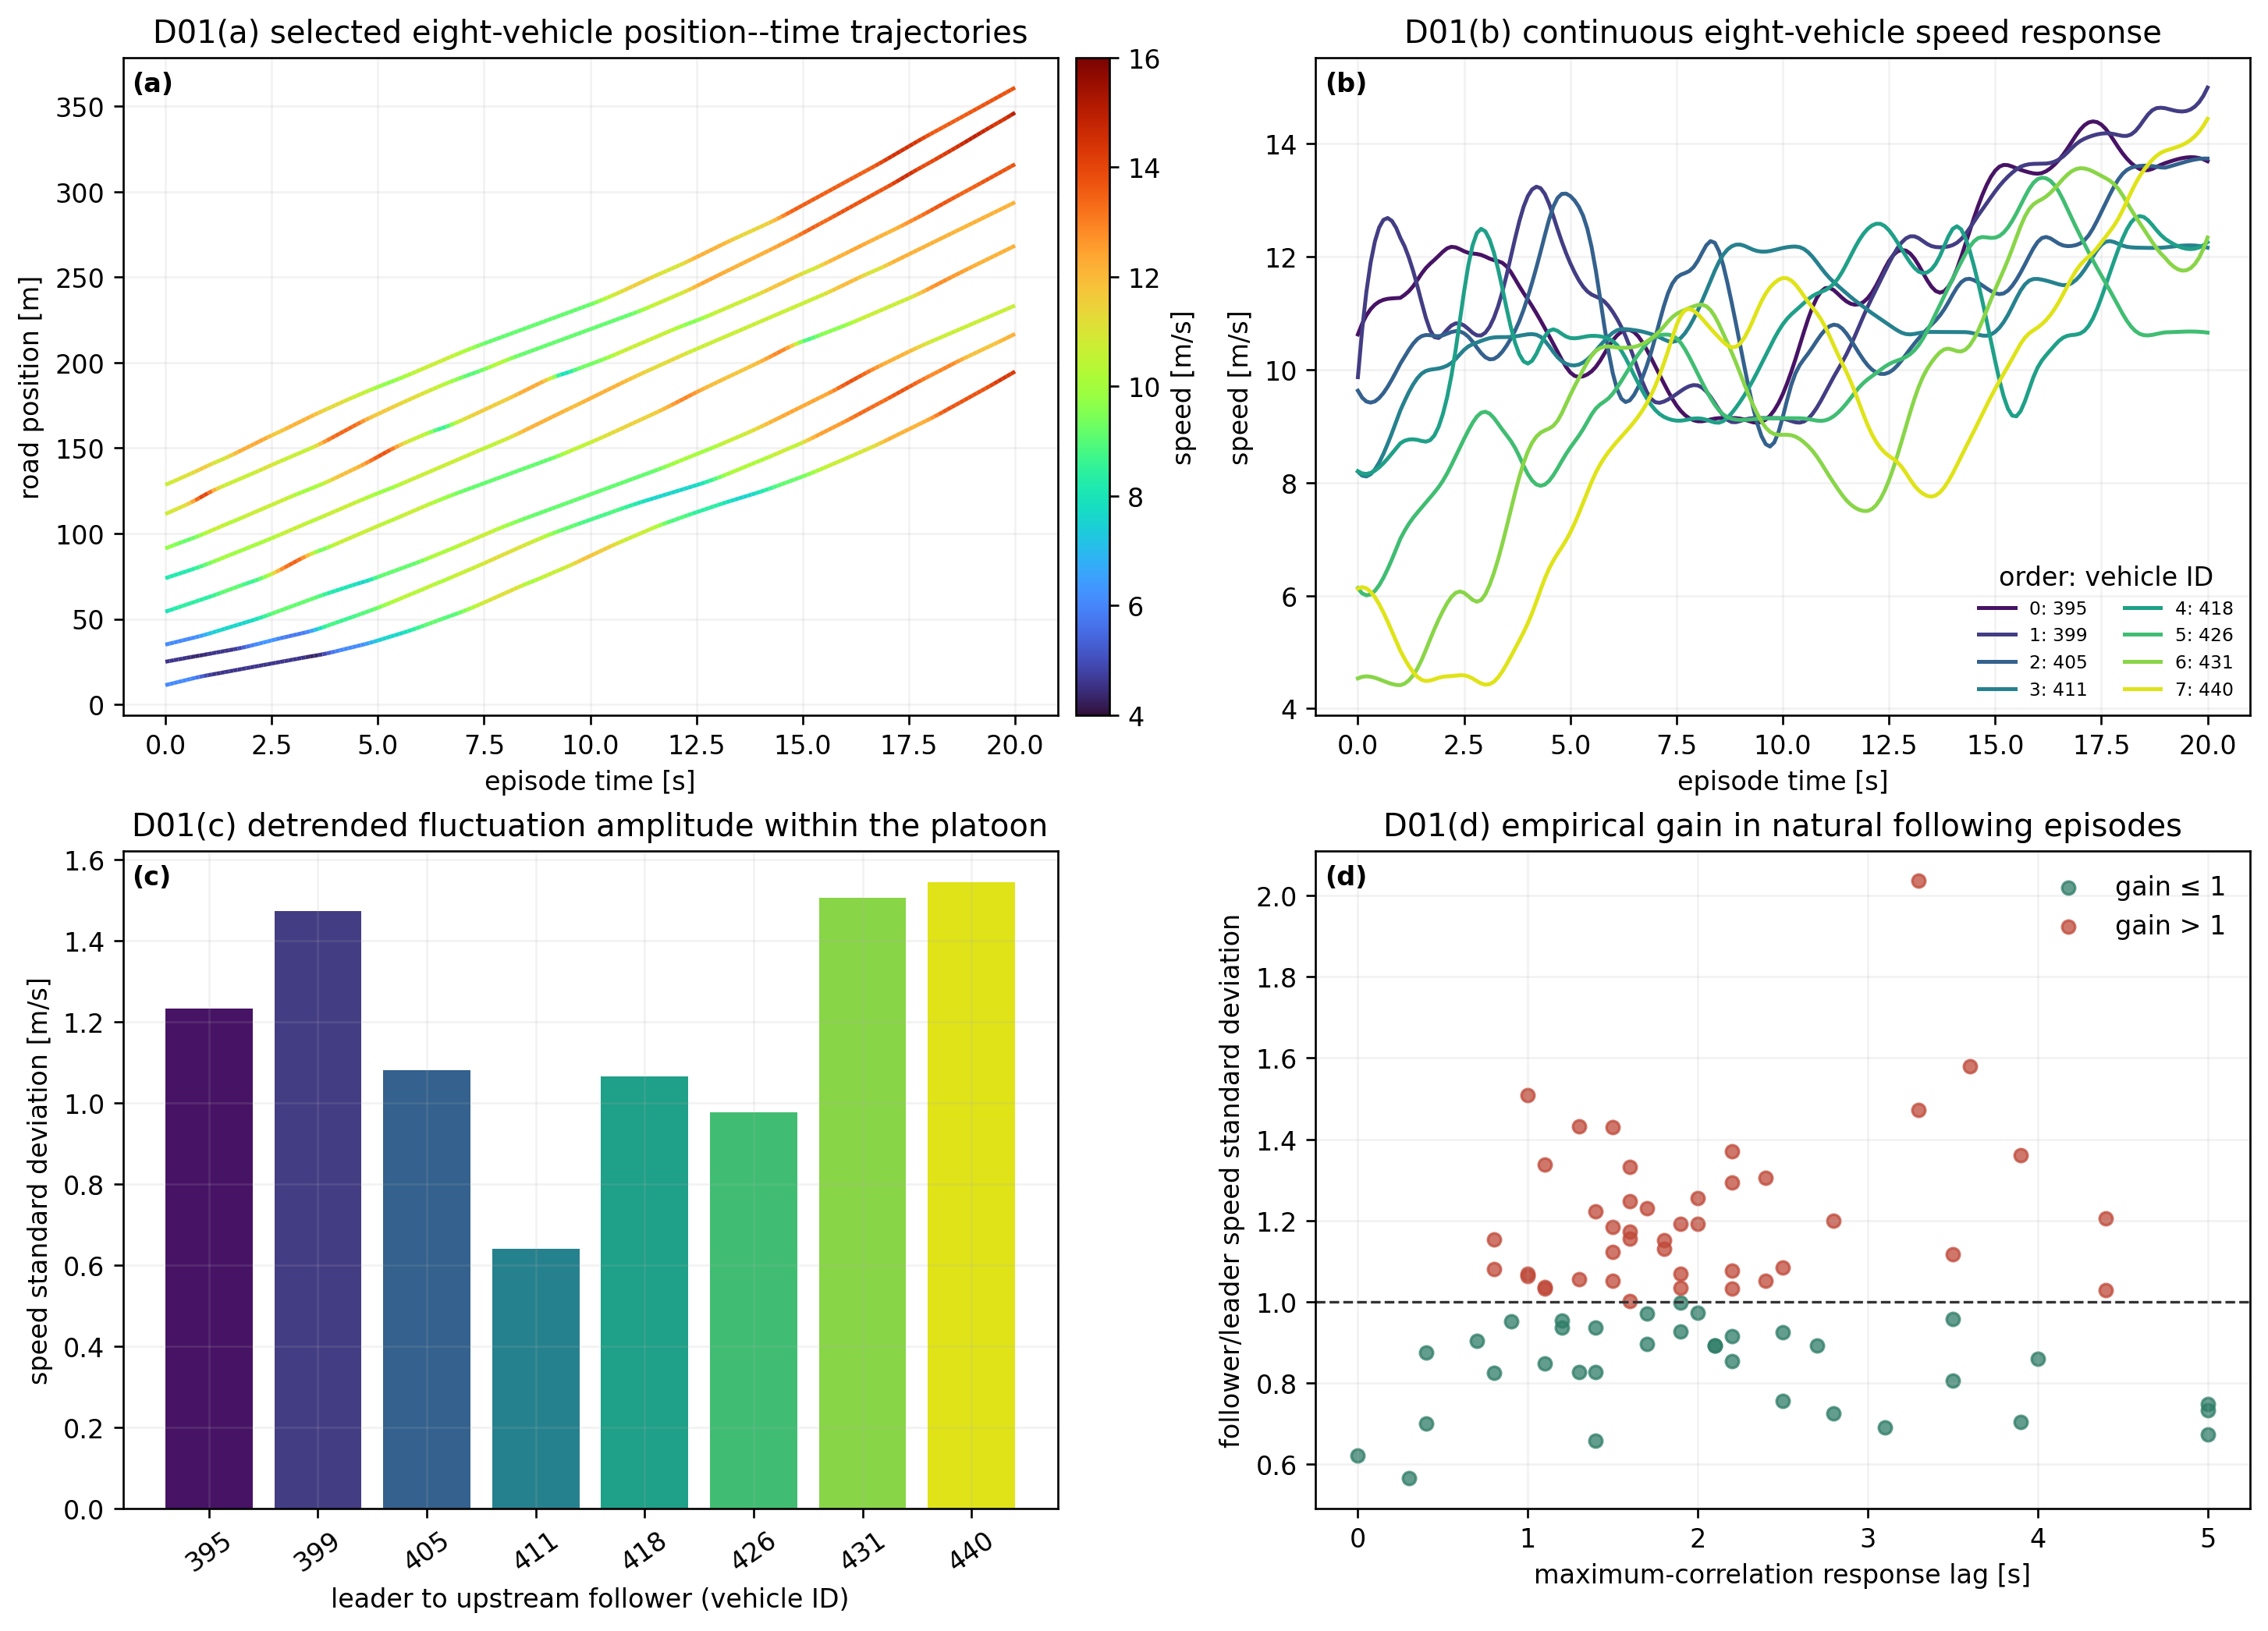
\includegraphics[width=\textwidth]{../../code/figures/ngsim_us101_d01_en.png}
\caption{D01: NGSIM trajectory-based propagation diagnosis.}\label{fig:ngsim-d01}
\end{figure}
Figure~\ref{fig:ngsim-d01} provides the whole evidence chain. Panel (a) first locates coherent speed disturbances in physical position--time coordinates. Panel (b) resolves the eight-vehicle chain, where peak and trough timing shifts upstream. Panel (c) shows why an endpoint-only gain is misleading: intermediate damping coexists with later amplification. Panel (d) aggregates the 78 episode gains and lags; red marks are amplification observations, not collision-risk labels. The figure therefore motivates stability-aware calibration while preserving its statistical uncertainty.

\section{D02: stability-aware calibration, validation, and design}
D02 uses the same eight-vehicle chain. The first 12 s are calibration data; the final 8 s are held out. Speeds and headways use the same filter as D01 and a 4.8-m vehicle length is subtracted to form net gap. To limit non-identifiability in this short record, $v_0=33.3$ m/s and $\delta=4$ are fixed; the estimated IDM parameters are $\theta=(T,s_0,a,b)$.

The conventional one-vehicle objective fits only vehicle 399,
\begin{equation}
J_{\rm one}=\frac{\operatorname{RMSE}(v_{399}^{\rm sim},v_{399}^{\rm obs})}{1\ \mathrm{m/s}}
+\frac{\operatorname{RMSE}(s_{399}^{\rm sim},s_{399}^{\rm obs})}{5\ \mathrm{m}},
\end{equation}
whereas the platoon objective fits all seven followers and the spatial fluctuation profile,
\begin{equation}
J_{\rm platoon}=\frac{\operatorname{RMSE}(\bm v^{\rm sim},\bm v^{\rm obs})}{1\ \mathrm{m/s}}
+\frac{\operatorname{RMSE}(\bm s^{\rm sim},\bm s^{\rm obs})}{5\ \mathrm{m}}
+1.25\operatorname{RMSE}(\log\bm A^{\rm sim},\log\bm A^{\rm obs}),
\label{eq:ngsim-platoon-objective}
\end{equation}
with $A_j=\operatorname{std}\{\operatorname{detrend}[v_j(t)]\}$. The final term preserves the shape of disturbance propagation, not simply more pointwise samples.

\begin{table}[htbp]\centering
\caption{D02 IDM calibration and replay results.}\label{tab:d02-calibration}
\begin{tabular}{lrrrrrr}\toprule
Objective & $T$ (s) & $s_0$ (m) & $a$ (m/s$^2$) & $b$ (m/s$^2$) & $\Phi$ (s$^{-2}$) & train $v$ RMSE\\\midrule
Single vehicle & 0.4458 & 6.000 & 2.257 & 4.500 & $-0.25942$ & 3.058\\
Platoon/stability & 0.9474 & 6.000 & 1.550 & 0.500 & $+0.04321$ & 1.104\\\bottomrule
\end{tabular}\end{table}

Table~\ref{tab:d02-calibration} makes the substantive point: a locally acceptable trajectory fit can imply the opposite long-wave sign. Parameters at their bounds also warn that this short episode does not uniquely identify driving behavior. On the 8-s held-out recursive simulation, the platoon calibration reduces speed RMSE from 2.782 to 0.845 m/s and net-gap RMSE from 4.429 to 2.904 m; its amplitude-profile error changes from 0.369 to 0.373 m/s. This is intentionally a mixed result: trajectory rollout improves clearly, while every propagation statistic is not automatically improved in a short validation window.

For a model-based controller design, use the fifth-percentile observed speed $v_{5\%}=6.185$ m/s and solve on a 60-vehicle ring
\begin{equation}
\min_{0\le\kappa\le0.5}\ \kappa\quad\text{s.t.}\quad
\max_{m\ne0}\Rea\lambda_m(v_{5\%},\kappa)\le-0.002\ \mathrm{s}^{-1}.
\end{equation}
The discrete search gives $\kappa^*=0.04$. In the corresponding 600-s counterfactual ring simulation, $\sigma_v(600)/\sigma_v(0)$ falls from 0.2767 to 0.1034. This control result belongs to the calibrated model, not to the historical road data; replaying the controller against the held-out leader input is only a sanity check, not observed deployment evidence.

\begin{figure}[htbp]\centering
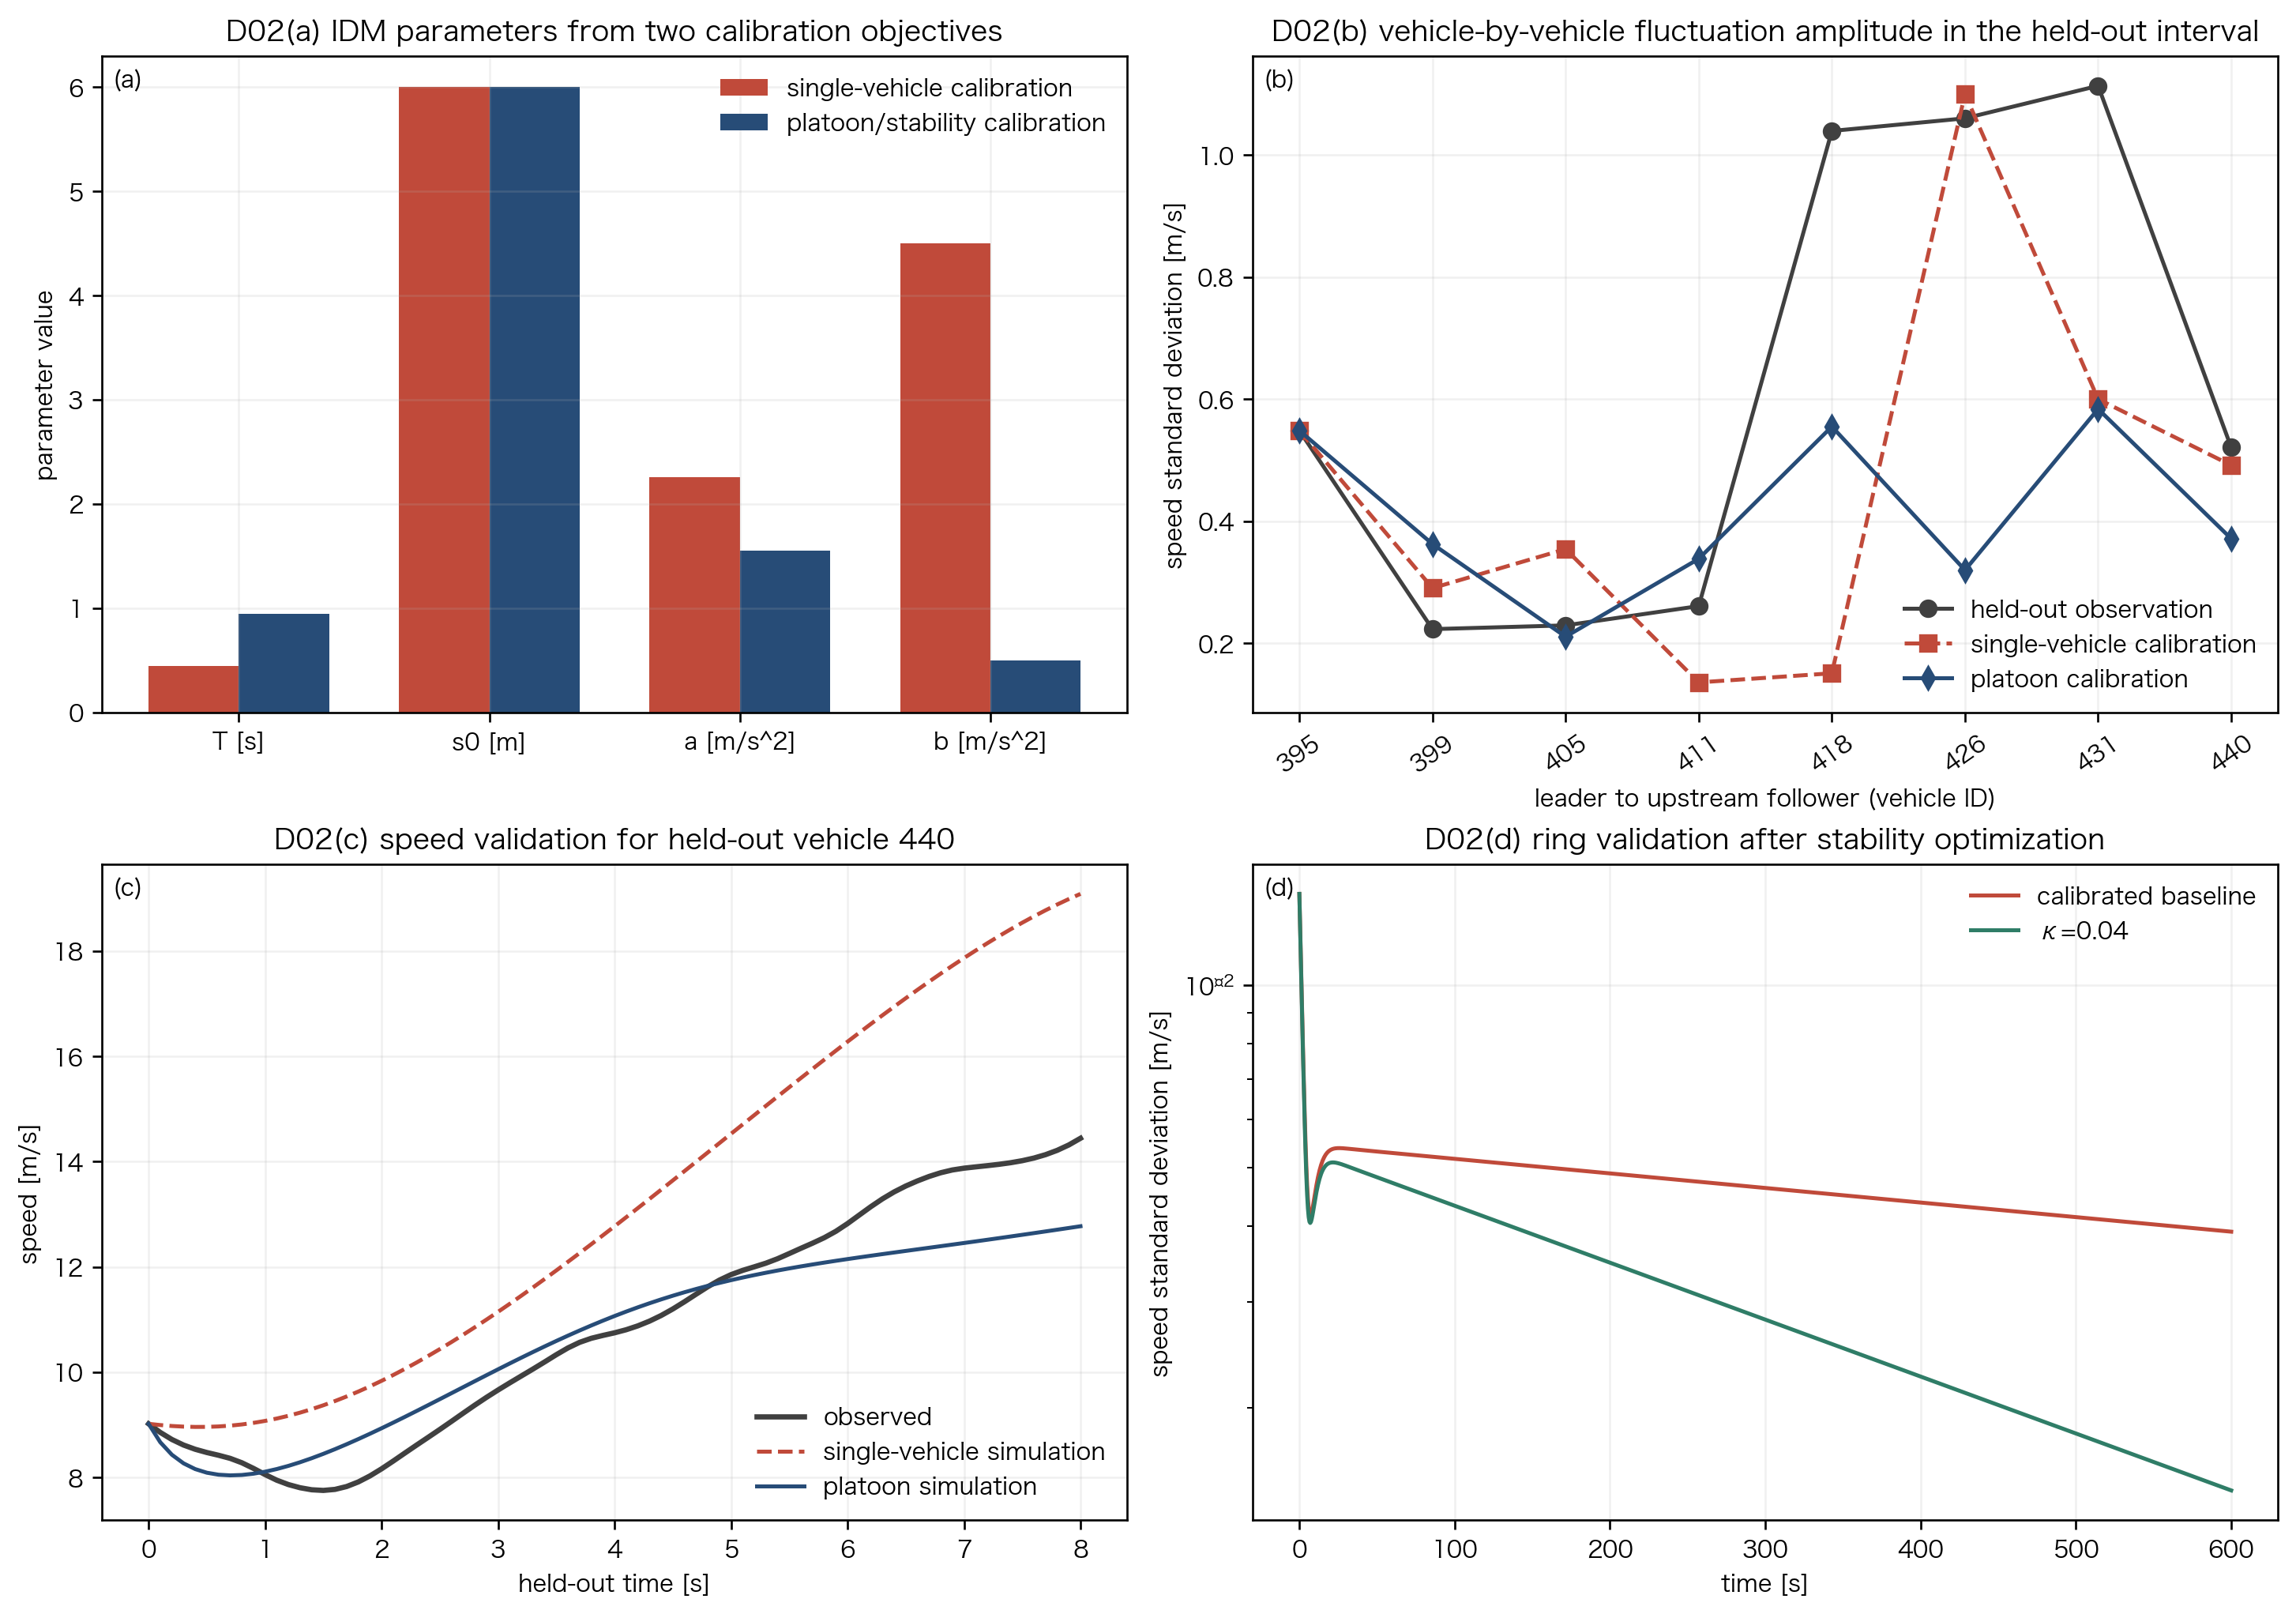
\includegraphics[width=\textwidth]{../../code/figures/ngsim_stability_application_d02_en.png}
\caption{D02: stability-aware calibration, held-out rollout, and model-based control.}\label{fig:ngsim-d02}
\end{figure}
Figure~\ref{fig:ngsim-d02} distinguishes the three evidence levels visually. The calibration panels show that using an amplitude profile changes the fitted IDM dynamics. The held-out panels show recursive, rather than frame-corrected, prediction. The final spectral panel selects a minimum intervention at a dangerous speed and checks it in a controlled ring. It demonstrates a workflow, not a claim that an AV controller was tested on US--101.

\chapterend{Real-data stability analysis is a chain of evidence: traceable preprocessing, episode-level propagation statistics, a stability-aware objective, genuinely recursive held-out validation, and an explicitly labelled model counterfactual.}

\chapter{Application A: Disturbance Rejection in an Open Platoon}
\chapterguide{A finite sinusoidal input illustrates how cooperative AV information changes forced amplification, recovery, and the simulated safety, efficiency, and energy consequences.}

Consider an open 60-vehicle platoon in a uniform but string-unstable IDM state at $v_e=8$ m/s. The lead vehicle is the only external input:
\begin{equation}
v_0(t)=v_e+0.6\sin\!\left[\frac{2\pi(t-100)}{48}\right],\qquad100\le t\le340\ \mathrm{s}.
\label{eq:application-leader-sine}
\end{equation}
This 0.6-m/s, 48-s-period excitation lasts exactly five cycles. Its frequency is near the baseline peak-gain region, so an HDV platoon amplifies it upstream even after the input ends.

The cooperative comparison uses three-predecessor acceleration feedforward plus a follower-speed term,
\begin{equation}
\dot v_n=F_n+\sum_{j=1}^{3}\kappa\alpha^{j-1}\dot v_{n-j}
+\gamma\sum_{j=1}^{3}\alpha^{j-1}(v_{n-j}-v_n)+\eta(v_{n+1}-v_n),
\label{eq:application-cooperative-av}
\end{equation}
with $\kappa=0.34$, $\alpha=0.52$, $\gamma=0.045$, and $\eta=0.055$ where neighboring vehicles exist. The imposed leader trajectory is identical in both runs. Any difference is therefore a propagation effect, rather than a different demand pattern.

\begin{table}[htbp]\centering
\caption{Application A: simulated benefits under the identical lead-vehicle input.}\label{tab:application-av-benefits}
\begin{tabular}{lrr}\toprule
Metric & HDV/IDM & Cooperative AV\\\midrule
Last-vehicle speed amplitude (m/s) & 0.927 & 0.099\\
End-to-end propagation gain & 1.545 & 0.165\\
Peak speed standard deviation (m/s) & 0.549 & 0.193\\
Recovery time (s) & 454 & 392\\
Minimum net gap (m) & 12.59 & 13.11\\
Minimum TTC (s) & 65.3 & 116.2\\
Disturbance-added EV energy (Wh/vehicle) & 0.718 & 0.076\\\bottomrule
\end{tabular}\end{table}

For the energy post-evaluation, use the longitudinal EV model of Wu et al. \cite{wu2015} with tractive force
\begin{equation}
F_{\rm tr}=ma+kv^2+f_{\rm rl}mg+mg\sin\theta,
\end{equation}
and battery-side power
\begin{equation}
P_{\rm EV}=\frac{rR^2}{K^2}F_{\rm tr}^2+v(kv^2+f_{\rm rl}mg+mg\sin\theta)+mav,
\qquad E_{\rm EV}=\int_0^{T_f}P_{\rm EV}\dd t.
\label{eq:wu-ev-power}
\end{equation}
The calculation uses $m=1266$ kg, $f_{\rm rl}=0.006$, $k=1.30$ kg/m, $K=10.08$ V s, $r=0.11\ \Omega$, $R=0.50$ m, and $\theta=0$. ``Disturbance-added'' energy is the trajectory energy minus the energy of the same vehicle traveling at 8 m/s for 1200 s. It isolates repeated acceleration/braking losses; it must not be reported as a universal production-EV consumption value.

\begin{figure}[htbp]\centering
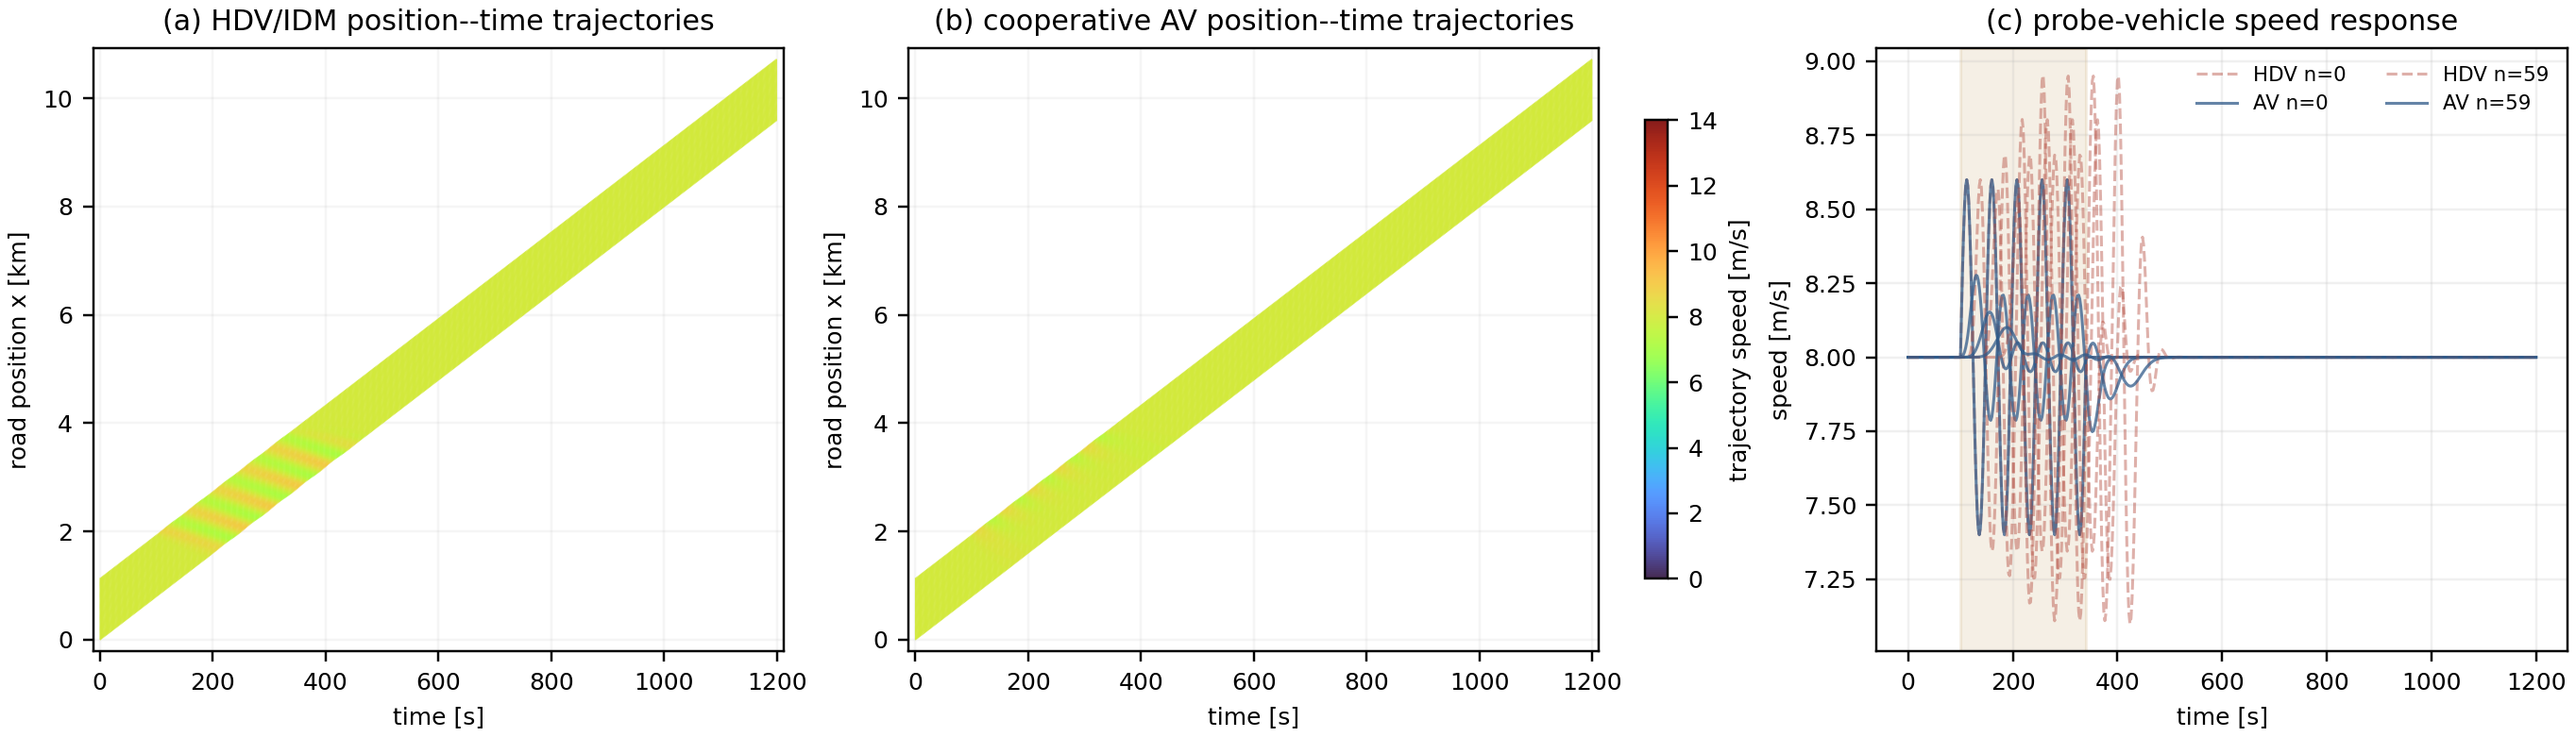
\includegraphics[width=\textwidth]{application_open_platoon_en.png}
\caption{Application A: cooperative AV disturbance rejection in an open platoon.}\label{fig:application-open-platoon}
\end{figure}
In Figure~\ref{fig:application-open-platoon}, the two position--time diagrams use the same speed color range and physical-road coordinate. The HDV bands broaden along the platoon and survive after the fifth forcing cycle. The cooperative case narrows the bands and returns sooner to nearly uniform colored trajectories. The probe traces make the visual comparison quantitative: Table~\ref{tab:application-av-benefits} reports an 89.3\% amplitude reduction and a 62-s earlier recovery. Gap, TTC, and energy are nonlinear simulation outcomes; the linear mechanism is the suppressed transfer gain.

\chapterend{Cooperative feedback is useful when it reduces both forced amplification and post-forcing recovery. The spectrum identifies the mechanism; safety, delay, comfort, and energy require separate nonlinear trajectory evaluation.}

\chapter{Event-Triggered Variable Speed Limits}
\chapterguide{This corrected experiment uses continuous inflow, a fixed one-kilometer upstream control zone, a 120 km/h statutory limit, and no anticipatory control before the slow vehicle appears.}

Consider a single-lane road with continuous arrivals over $0$--$1200$ s. To make the uncontrolled state genuinely string unstable, use the baseline IDM parameters except a deliberately short desired headway $T=0.7$ s. At net gap $s_e=18$ m and the statutory desired speed $v_0=120$ km/h, the uniform equilibrium is $v_e=74.95$ km/h, flow is about 3261 veh/h, and $\Phi=-0.001415\ \mathrm{s}^{-2}$. This is a high-demand theoretical operating point, not a typical single-lane human-driver capacity estimate. A slow vehicle arrives near $x_b=6$ km at
\begin{equation}
t_{\mathrm{incident}}=300\ \mathrm{s}.
\end{equation}
Vehicle 533 reduces its target speed to 18 m/s from $t=300$ to $420$ s, creating a finite bottleneck disturbance. The VSL zone is fixed in road coordinates over the one-kilometer segment immediately upstream of the incident point,
\begin{equation}
\Omega_{\rm VSL}=[x_b-1000,x_b)=[5000,6000)\ \mathrm{m},\qquad300\le t\le900\ \mathrm{s}.
\label{eq:vsl-fixed-zone}
\end{equation}
It is never attached to the moving vehicle. Before 300 s, the statutory limit is 120 km/h and the VSL controller is strictly off. At the incident time it is activated and ramped over 30 s, then released smoothly from 810 to 900 s. This timing prevents the invalid comparison in which controlled traffic is preconditioned before the disturbance exists.

\section{Why a lower speed limit can stabilize flow}
For each permitted target $u\in[114,120]$ km/h, reset the IDM desired speed to $v_0=u$, solve
\begin{equation}
F(s_e,v_e(u),0;v_0=u,T=0.7\ \mathrm{s})=0,
\end{equation}
and calculate the long-wave margin
\begin{equation}
\Phi(u)=\frac12[f_v(u)^2-f_{v_l}(u)^2]-f_s(u).
\label{eq:vsl-phi}
\end{equation}
The online design uses stability only,
\begin{equation}
u^*=\arg\max_{u\in[114,120]\ \mathrm{km/h}}\Phi(u).
\label{eq:vsl-stability-only-objective}
\end{equation}
This intentionally maximizes the available stability margin, as requested. Queue length, TTC, delay, and energy remain post-simulation evaluations, rather than unavailable online objectives.

\begin{table}[htbp]\centering\caption{VSL candidates recalculated at the same 18-m net gap.}\label{tab:vsl-candidates}
\begin{tabular}{rrrr}\toprule
$u$ (km/h) & $v_e(u)$ (km/h) & $\Phi(u)$ (s$^{-2}$) & conclusion\\\midrule
114 & 73.78 & $+0.002396$ & stable; maximum margin\\
115 & 73.98 & $+0.001727$ & stable\\
116 & 74.19 & $+0.001071$ & stable\\
117 & 74.39 & $+0.000429$ & stable\\
118 & 74.58 & $-0.000199$ & unstable\\
119 & 74.77 & $-0.000814$ & unstable\\
120 & 74.95 & $-0.001415$ & unstable\\\bottomrule
\end{tabular}\end{table}
Table~\ref{tab:vsl-candidates} selects $u^*=114$ km/h. The six-km/h reduction is not chosen after looking at safety or delay; it moves the local upstream operating point from the unstable to the stable side while maximizing the prescribed analytical margin inside the operational speed band.

Reducing desired speed upstream can lower the inflow to the bottleneck, reduce speed differences at the queue tail, and move the local operating point from an unstable branch into a stable region. A useful design must produce an upstream-moving congestion front in the uncontrolled case and demonstrate that event-triggered VSL weakens that front rather than simply moving traffic more slowly everywhere.

\section{Corrected results}
The corrected simulation uses identical arrivals and slow-vehicle timing in both runs. Table~\ref{tab:vsl} reports the principal measurements.
\begin{table}[htbp]
\centering
\caption{Corrected event-triggered VSL results.}
\label{tab:vsl}
\begin{tabular}{lrrr}
\toprule
Metric & No VSL & Event-triggered VSL & Change\\
\midrule
Queue-tail speed (m/s) & $-2.687$ & $-0.284$ & $89.4\%$ weaker\\
Peak queued vehicles & $121$ & $102$ & $15.7\%$ lower\\
Peak speed standard deviation (m/s) & $8.912$ & $4.107$ & $53.9\%$ lower\\
Minimum gap (m) & $1.56$ & $3.27$ & $109.8\%$ higher\\
Minimum TTC (s) & $2.34$ & $6.70$ & $186\%$ higher\\
Total delay (veh h) & $6.866$ & $4.799$ & $30.1\%$ lower\\
EV energy intensity & $17.521$ & $17.328$ & $1.10\%$ lower\\
\bottomrule
\end{tabular}
\end{table}
Define the congestion-tail location as $x_q(t)=\min\{x_n(t):v_n(t)<18.2\ \mathrm{m/s}\}$ and fit $c_q=\dd x_q/\dd t$ on 360--420 s. The uncontrolled $c_q=-2.687$ m/s is an upstream-moving queue tail. With VSL it is $-0.284$ m/s: the control weakens, rather than reverses by declaration, the nonlinear queue-wave formation. The safety, delay, and energy figures in Table~\ref{tab:vsl} are downstream consequences of the same simulation. The bilingual laboratory exposes the event markers so the green control band begins at exactly $t=300$ s.

\begin{figure}[htbp]\centering
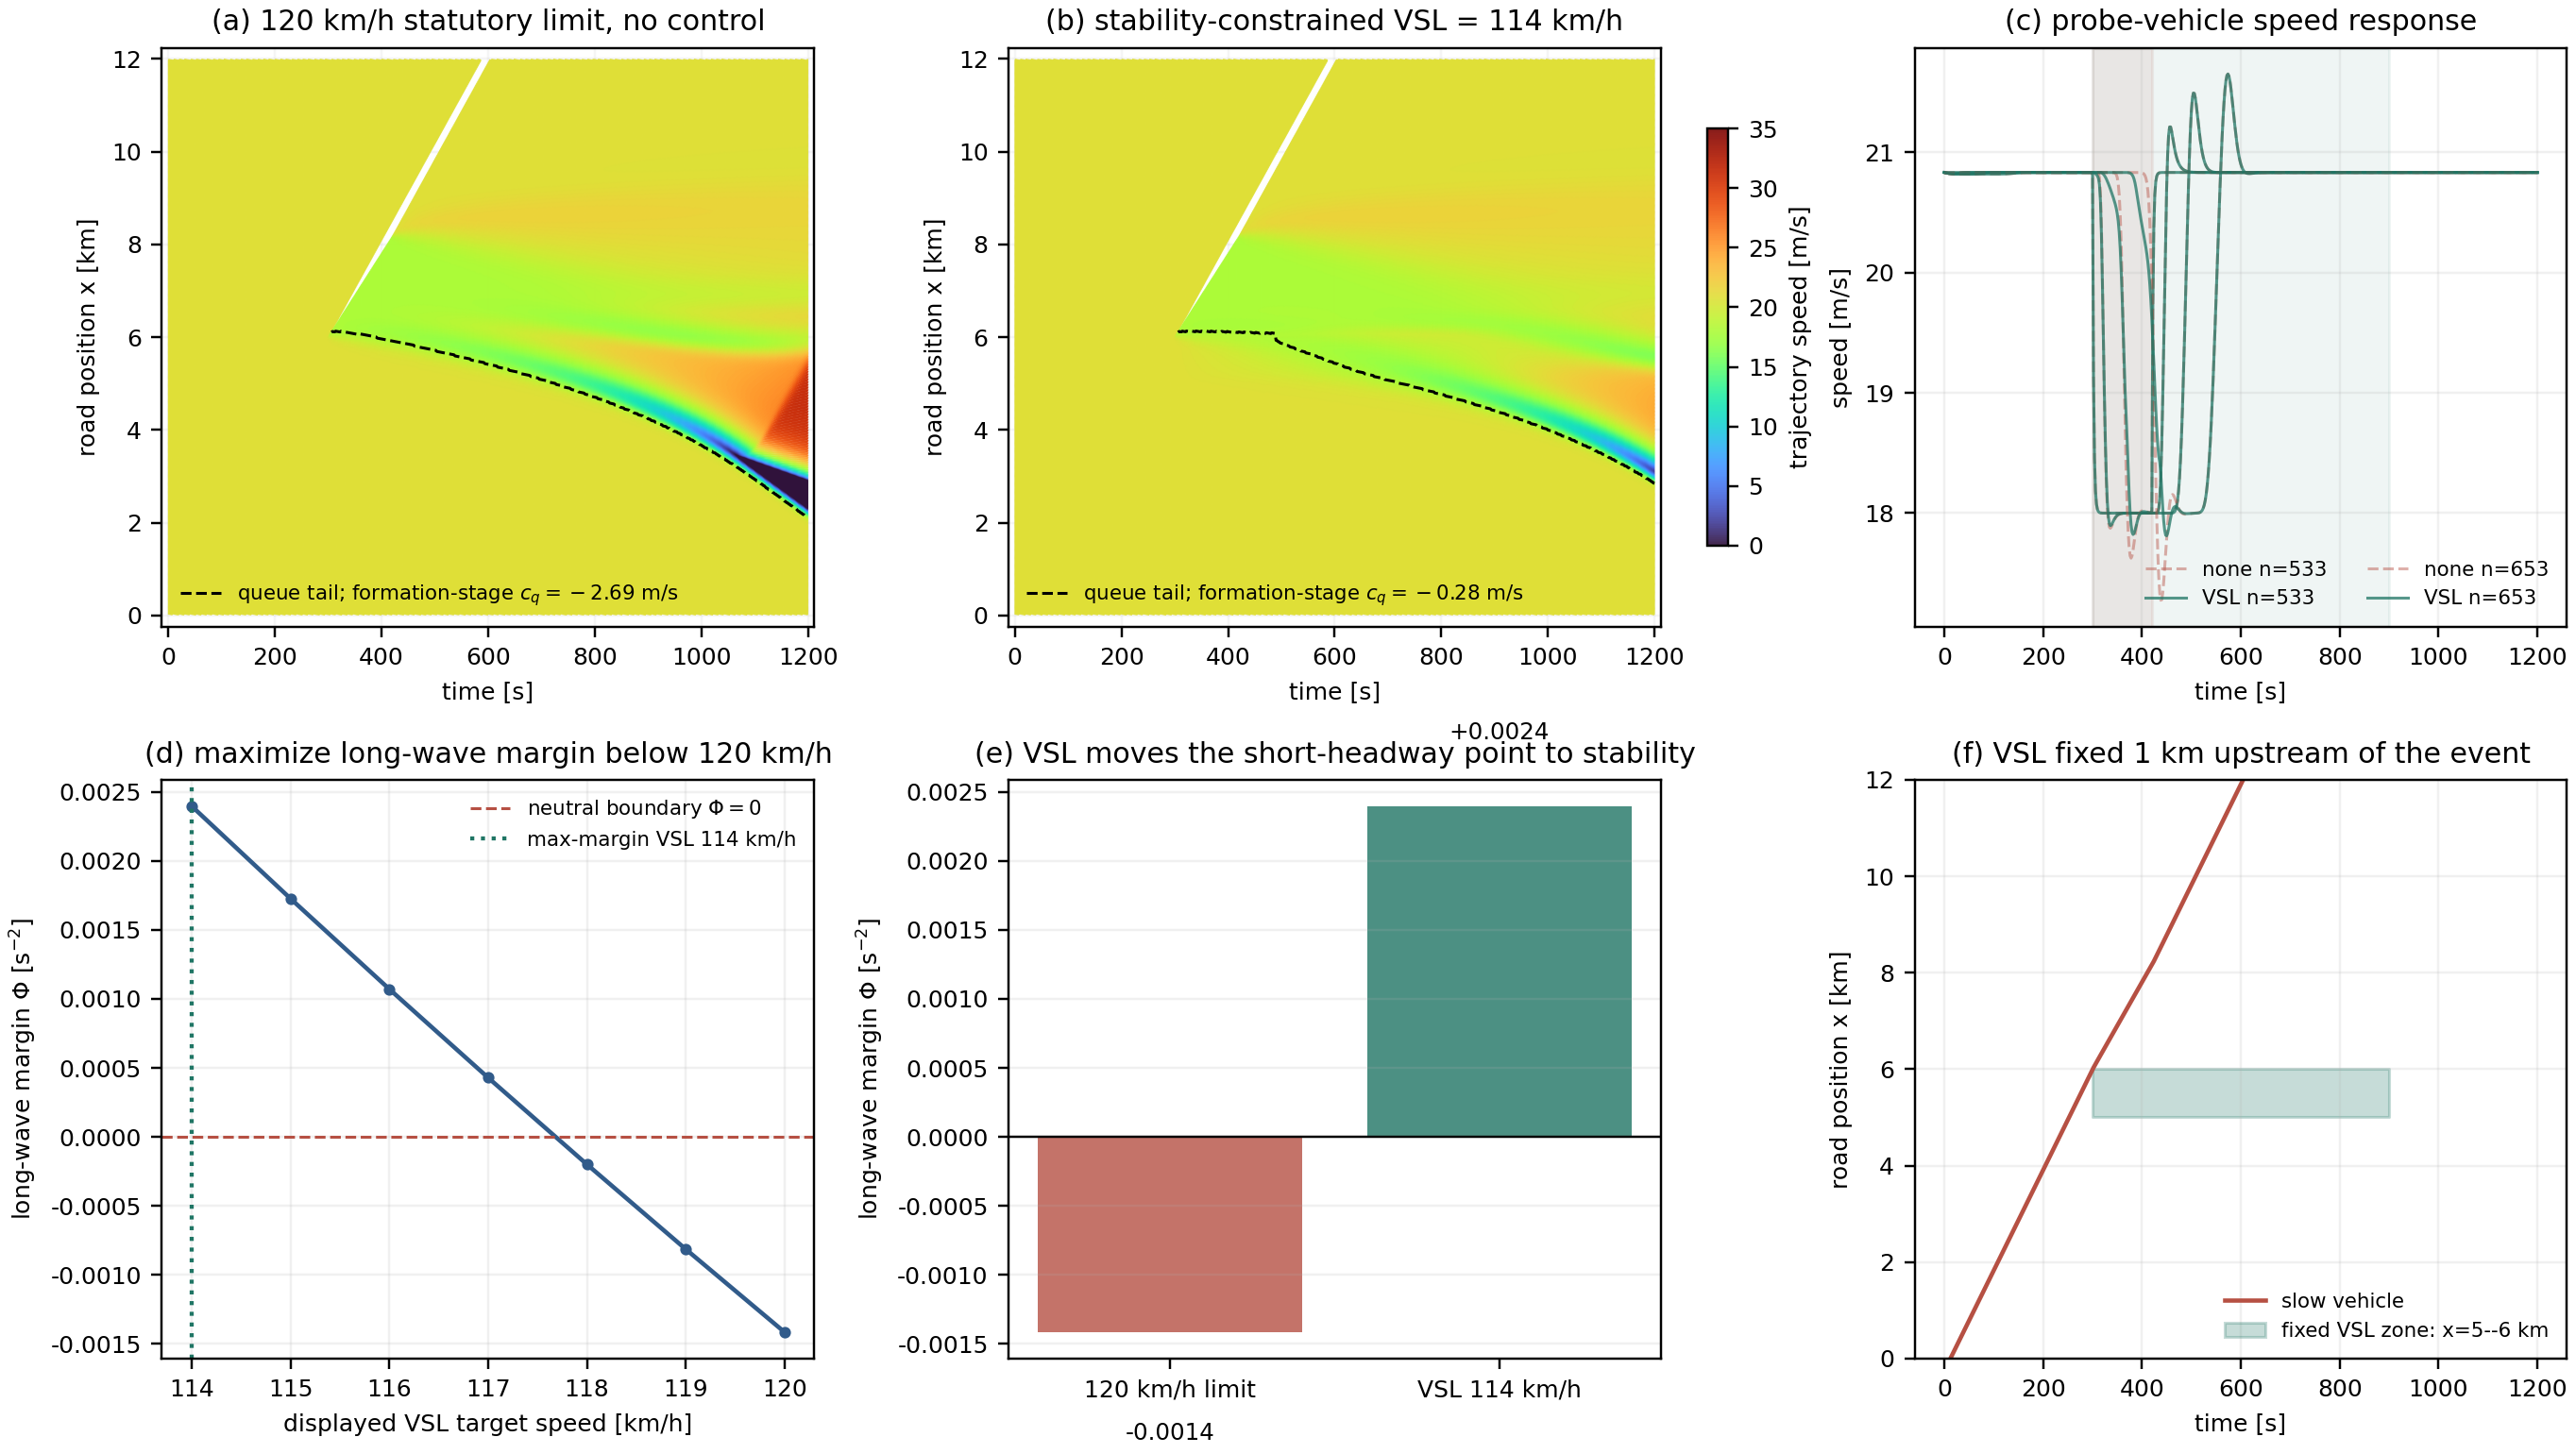
\includegraphics[width=\textwidth]{application_moving_bottleneck_en.png}
\caption{Application B: fixed-zone, event-triggered VSL chosen by stability margin.}\label{fig:application-moving-bottleneck}
\end{figure}
Figure~\ref{fig:application-moving-bottleneck} separates time from space. The VSL band remains fixed over 5--6 km while the slow-vehicle trajectory leaves the event location; the control is absent before 300 s. In the uncontrolled panel, the low-speed queue tail slopes toward smaller $x$, directly displaying upstream propagation. After trigger, the narrower low-speed band and flatter queue-tail slope agree with the margin calculation in Table~\ref{tab:vsl-candidates}. The visual result is supported by the quantitative post-evaluation in Table~\ref{tab:vsl}, not substituted for it.

\chapterend{The VSL becomes active only when the slow-vehicle disturbance begins. Its mechanism is to reshape the upstream operating point and reduce speed mismatch, not to anticipate an event that has not occurred.}

\chapter{Machine Learning and Deep Learning Stability}
\chapterguide{Prediction accuracy does not certify dynamic stability. The correct stability object depends on the learned architecture, hidden state, graph, sample-and-hold rule, and closed-loop deployment semantics.}

\section{Four meanings of stability in a learning problem}
``Stable learning'' can mean optimization converges, a one-step predictor has bounded error, a recurrent rollout stays bounded, or traffic perturbations decay along a platoon. Only the final meaning is the object of this book. A model trained on realistic human-driver data should reproduce observed amplification where it exists; an AV controller should suppress amplification over its specified operating domain. These are different targets and should not be conflated by adding a generic ``stability loss.''

For a differentiable learned acceleration $a_\theta=F_\theta(s,v,\Delta v,z)$, first solve the complete equilibrium $F_\theta(s_e,v_e,0,z_e)=0$ together with the hidden-state fixed-point condition. Automatic differentiation then recovers the physical Jacobian entries. Classical local and string criteria can be used only when the deployed mapping is Markovian and vehicle-local. A sampled discrete controller must instead be tested relative to the unit disk, not the continuous-time left half plane.

\section{Architecture determines the linearization}
An MLP or neural residual car-following law has a scalar vehicle Jacobian and can be substituted into the derivatives of Chapters 3--4. RNNs, LSTMs, Neural ODEs, and delay embeddings require an augmented state $(s,v,z)$ and the full recurrent Jacobian. GNNs and attention models require a graph-level Jacobian or spatial transfer operator: a scalar predecessor gain is generally insufficient. A reinforcement-learning reward is not a Lyapunov certificate, because the policy, measurement filter, action hold, saturation, and vehicle dynamics form the actual closed loop.

At an equilibrium grid, a stability-aware loss can combine trajectory error with penalties on equilibrium error, positive spectral abscissa, and excessive gain:
\begin{equation}
\mathcal L=\mathcal L_{\mathrm{data}}+\lambda_e\mathcal L_{\mathrm{eq}}
+\lambda_s\bigl[\max(0,\alpha(J))\bigr]^2
+\lambda_g\int\bigl[\max(0,|G(i\omega)|-1)\bigr]^2\dd\omega.
\end{equation}
For a graph or recurrent model, replace $G$ by the maximum eigenvalue, singular gain, or full modal spectral abscissa appropriate to that architecture. Training points should include equilibrium states that are physically feasible but scarce in the data; otherwise an accurate model can retain incorrect derivatives just outside the recorded distribution.

\section{Worked example ML01: identical equilibrium prediction, opposite propagation}
Consider the three-neuron toy law
\begin{equation}
\widehat F=c_s\tanh\frac{s-s_e}{10}+c_v\tanh\frac{v-v_e}{5}+c_\Delta\tanh\frac{\Delta v}{5}.
\end{equation}
Both models below output zero at $(s_e,v_e,0)$, so equilibrium acceleration data alone cannot distinguish them.
\begin{table}[htbp]\centering\caption{ML01 automatic-differentiation stability diagnosis.}\label{tab:ml01}
\begin{tabular}{lrrrrrr}\toprule
Network & $c_s$ & $c_v$ & $c_\Delta$ & $F_s$ & $f_v$ & $\Phi$ (s$^{-2}$)\\\midrule
A: trajectory-only & 0.42 & -0.50 & -0.90 & 0.042 & -0.280 & -0.019\\
B: stability-aware & 0.34 & -0.80 & -1.10 & 0.034 & -0.380 & +0.014\\\bottomrule
\end{tabular}\end{table}
At $\tanh'(0)=1$, model A has $F_{\Delta v}=-0.180$, $f_{v_l}=0.180$, and $\Phi_A=\tfrac12(0.28^2-0.18^2)-0.042=-0.019$. Model B has $F_{\Delta v}=-0.220$, $f_{v_l}=0.220$, and $\Phi_B=+0.014$. Both may be locally stable, yet only B is long-wave stable. Table~\ref{tab:ml01} is a teaching construction, not a real-data training result; it demonstrates why zero error at a point carries no derivative information.

\section{From diagnostic scan to certificate}
Spectral normalization and contraction penalties can bound a network Lipschitz constant, roughly by the product of layer spectral norms. This is useful during training but often conservative and does not alone prove closed-loop string stability. A neural Lyapunov certificate requires a specified state domain $\Omega$, $V_\phi(x)>0$ for $x\ne x_e$, and $\nabla V_\phi^\top f_{\rm cl}<0$ throughout that domain, with a verifier or counterexample search rather than finite training samples alone. IQC/SDP and reachability methods can provide stronger regional claims at substantially higher computational cost.

\begin{table}[htbp]\centering\caption{A reproducible six-experiment program for learned traffic models.}\label{tab:ml-experiments}
\begin{tabular}{p{1cm}p{3.3cm}p{7.4cm}}\toprule
ID & Object & Required evidence\\\midrule
ML01 & differentiable MLP & derivative grid, $\Phi$, and full-frequency gain\\
ML02 & stability-aware training & RMSE--worst-margin Pareto frontier\\
ML03 & RNN/LSTM & augmented Jacobian, 1800-s rollouts, hidden-state sensitivity\\
ML04 & GNN/attention & graph spectrum, singular gain, and vehicle-count/topology tests\\
ML05 & RL controller & complete closed-loop spectrum, recovery, saturation, and safety-filter activations\\
ML06 & certificate search & certified region, tolerance, and the first counterexample outside it\\\bottomrule
\end{tabular}\end{table}
Claims must remain architecture-specific: a finite sampled-Jacobian scan is a local diagnostic; a verified Lyapunov or reachability proof supports a stated region; neither is an all-road, all-vehicle global certificate.

\chapterend{Learned traffic models need dynamical validation in addition to predictive validation. Specify the full deployed state, linearize the appropriate architecture, scan the relevant modes, and distinguish empirical rollouts from regional certificates.}

\chapter{Reproducibility and the Online Laboratory}
\chapterguide{The book, numerical cases, source code, machine-readable metrics, and browser laboratory form one reproducible package rather than independent presentations of the same idea.}

\section{One experiment, one definition}
Every reported experiment must record its parameter file, source commit, random seed, initial and boundary conditions, integrator, step size, raw or derived data, plot, and reference metrics. The stable identifiers M01--M06, W01--W03, D01--D02, and E1--E14 bind the relevant chapter, script entry point, JSON/CSV result, and figure. This prevents the common drift in which a page says $N=30$ while the plotted file still contains $N=60$.

\begin{verbatim}
traffic-stability-code/
|-- src/traffic_stability/   # models and solvers
|-- examples/                # W, M, D, and application entry points
|-- experiments/manifest.json
|-- tests/                   # scientific regression tests
|-- data/derived/            # compact, redistributable derived data
|-- results/                 # JSON/CSV metrics
`-- figures/                 # regenerated figures
\end{verbatim}

\section{What the first public results verify}
M01 records roots, period, overshoot, and RK4 error. M02 records the finite-ring rightmost roots for $N=12,20,30$. M03 records stable/unstable IDM theory versus measured growth. M04 records an intervention without state reset. M05 performs a step-size convergence check. M06 records the Rankine--Hugoniot shock comparison. W01--W03 preserve intermediate RK4 slopes and finite-volume fluxes; D01--D02 preserve derived trajectory statistics but not a redistributed full NGSIM archive.

\section{Re-run protocol}
From a clean Python 3.10+ environment, the intended workflow is
\begin{verbatim}
python3 -m venv .venv
source .venv/bin/activate
python -m pip install -e .
python examples/run_mini_examples.py
python examples/worked_update_examples.py
python examples/ngsim_stability_application.py
python -m unittest discover -s tests -v
\end{verbatim}
Scientific tests check more than executable syntax: equilibrium residuals, the opposite signs of the 8- and 25-m/s IDM margins, finite-ring wavelength selection, the effect of feedforward on the rightmost root, shock speed, and structured result files. A formal release removes old generated results, reruns the pipeline, compares JSON, recompiles the book, and records the dependency versions.

\section{Interactive and batch roles}
The browser laboratory is bilingual through the upper-right language control. It supports live intervention: feedback or control parameters can change without resetting the state, so a stop-and-go wave can be seen before and after stabilization. Animation is deliberately not the authority for published numbers. Batch scripts use declared step sizes, deterministic output sampling, and regression checks; the browser is for diagnosis, parameter intuition, and communicating the same verified scenarios.

\chapterend{Reproducibility requires a single source of truth for equations, parameters, event timing, and metrics. Interactive visualization and batch verification serve complementary, not interchangeable, roles.}

\appendix
\part{Appendices}

\chapter{Stability Criteria at a Glance}
For $\lambda^2+a_1\lambda+a_0=0$ with real coefficients, both roots have negative real parts iff $a_1>0$ and $a_0>0$. For a state matrix $A$, local asymptotic stability requires its spectral abscissa $\alpha(A)=\max_j\Rea\lambda_j(A)$ to be negative. For an open homogeneous chain, frequency-domain string stability requires $\sup_{\omega\ge0}|G(i\omega)|\le1$. A periodic ring instead evaluates only discrete spatial modes $k_j=2\pi j/N$.

For a complex quadratic, real-coefficient Routh--Hurwitz cannot be applied directly. A Bilharz determinant or an equivalent real $4\times4$ representation must be used. Multiplying the polynomial by a nonzero complex factor does not change its roots, but sign arguments may only discard a factor after proving that the discarded real factor is strictly positive.

\section{Vieta's relations and the complex quadratic}
For $z^2+c_1z+c_0=(z-z_1)(z-z_2)$, comparison of coefficients gives $z_1+z_2=-c_1$ and $z_1z_2=c_0$. Write two stable roots as
\begin{equation}
z_1=-\alpha_1+i\beta_1,\qquad z_2=-\alpha_2+i\beta_2,\qquad \alpha_1,\alpha_2>0.
\end{equation}
If $c_1=p_1+iq_1$ and $c_0=p_2+iq_2$, direct multiplication gives
\begin{align}
p_1&=\alpha_1+\alpha_2,&q_1&=-(\beta_1+\beta_2),\\
p_2&=\alpha_1\alpha_2-\beta_1\beta_2,&q_2&=-(\alpha_1\beta_2+\alpha_2\beta_1).
\end{align}
Substitution and collection yields the second Bilharz determinant
\begin{equation}
\Delta_2=p_1(p_1p_2+q_1q_2)-q_2^2
=\alpha_1\alpha_2\left[(\alpha_1+\alpha_2)^2+(\beta_1-\beta_2)^2\right].
\label{eq:bilharz-root-factor}
\end{equation}
Consequently, for a complex quadratic, both roots are strictly in the left half plane iff $p_1>0$ and $\Delta_2>0$. Equation~\eqref{eq:bilharz-root-factor} explains the criterion rather than treating it as a black box: the determinant enforces equal signs of $\alpha_1,\alpha_2$, and $p_1>0$ selects the positive pair.

\chapter{Full Algebra for Bilateral-Acceleration Conditions}
\chapterguide{This appendix expands the two conditions for the bilateral acceleration model, including every valid cancellation of a complex denominator.}

For a nontrivial spatial mode, write $u=\cos k$, $s_k=\sin k$, $\sigma=f_a+f_b$, and $d=f_a-f_b$. The bilateral characteristic equation is
\begin{equation}
P\lambda^2-Q\lambda-R=0,
\end{equation}
where
\begin{align}
P&=1-f_ae^{-ik}-f_be^{ik}=(1-\sigma u)+i(ds_k),\\
Q&=f_v+f_{v_l}e^{-ik}=(f_v+f_{v_l}u)-if_{v_l}s_k,\\
R&=f_s(e^{-ik}-1)=f_s(u-1)-if_ss_k.
\end{align}
Normalize by $P$ as $\lambda^2+c_1\lambda+c_0=0$, with $c_1=-Q/P=p_1+iq_1$ and $c_0=-R/P=p_2+iq_2$. Let
\begin{equation}
D(u)=|P|^2=(1-\sigma u)^2+d^2(1-u^2).
\end{equation}
The normalization is legitimate only when $P\ne0$, so $D>0$. Multiplying numerator and denominator by $\overline P$ gives
\begin{align}
p_1&=\frac{\Pi(u)}{D(u)},&q_1&=\frac{s_k\Xi(u)}{D(u)},\\
p_2&=\frac{f_s(1-u)\Gamma(u)}{D(u)},&q_2&=\frac{f_ss_k\Omega(u)}{D(u)},
\label{eq:bilateral-components}
\end{align}
where
\begin{align}
\Pi(u)&=-(f_v+f_{v_l}u)+\sigma f_vu+f_{v_l}(d+2f_bu^2),\\
\Xi(u)&=d(f_v+f_{v_l}u)+f_{v_l}(1-\sigma u),\\
\Gamma(u)&=1+d-2f_bu,\qquad \Omega(u)=1-d-2f_bu.
\end{align}
Thus the first Bilharz condition is simply $p_1>0\Leftrightarrow\Pi(u)>0$: $D$ may be cancelled because it is strictly positive, not merely because it appears on both sides.

For the second condition, use $s_k^2=(1-u)(1+u)$ in (\ref{eq:bilateral-components}):
\begin{align}
p_1(p_1p_2+q_1q_2)&=\frac{f_s(1-u)}{D^3}\Pi[\Pi\Gamma+(1+u)\Xi\Omega],\\
q_2^2&=\frac{f_s(1-u)}{D^3}[f_sD(1+u)\Omega^2].
\end{align}
Hence
\begin{equation}
\Delta_2=\frac{f_s(1-u)}{D^3}H(u),\quad
H=\Pi[\Pi\Gamma+(1+u)\Xi\Omega]-f_sD(1+u)\Omega^2.
\end{equation}
Collecting powers of $u$ gives the exact factorization $H(u)=D(u)\widetilde W(u)$, where
\begin{align}
\widetilde W(u)&=w_3u^3+w_2u^2+w_1u+w_0,\\
w_3&=-4f_b^2f_s,\\
w_2&=2f_b[2f_s(1-f_a)+f_{v_l}(f_{v_l}-f_v)],\\
w_1&=-f_s(1-\sigma)^2+4f_b^2f_s-\sigma f_v^2+(1+\sigma)f_vf_{v_l}-f_{v_l}^2,\\
w_0&=-f_s(1-d)^2+f_v^2-f_vf_{v_l}+df_{v_l}(f_{v_l}-f_v).
\end{align}
Therefore
\begin{equation}
\boxed{\Delta_2=\frac{f_s(1-u)}{D(u)^2}\widetilde W(u).}
\end{equation}
For $k\ne0$, $u<1$; with $f_s>0$ and $D>0$, the second Bilharz condition is exactly $\widetilde W(u)>0$. The two quick checks are $f_b=0$, for which the cubic reduces to a linear condition, and $f_a=f_b=0$, for which $P=D=1$ and the baseline long-wave condition is recovered as $u\to1$.

\chapter{Ring Modes and Transfer Functions}
\chapterguide{This appendix connects the open-chain gain to ring-road eigenmodes and explains what finite vehicle number changes.}

For a uniform predecessor-following linearization, the Laplace-domain vehicle relation is $Y_n(\lambda)=G(\lambda)Y_{n-1}(\lambda)$. On a periodic ring, traveling once around the vehicle labels must return to the same perturbation:
\begin{equation}
\prod_{n=1}^NG_n(\lambda)=1.
\end{equation}
If all vehicles are identical, $G_n=G$, so $G(\lambda)^N=1$. The $N$th roots of unity are $e^{ik_m}$ with $k_m=2\pi m/N$, hence
\begin{equation}
G(\lambda)=e^{ik_m}.
\end{equation}
Taking moduli at a marginal mode gives $|G|=1$. In an open chain, the stronger all-frequency requirement $|G(i\omega)|\le1$ prevents any harmonic input from growing vehicle by vehicle. The ring identity alone does \emph{not} imply that every factor or every partial product is no larger than one; it only closes the product after one entire circuit. In a heterogeneous open platoon, every prefix must be monitored. In a heterogeneous ring, the total product is constrained by periodic closure, but individual segments may have large transient amplification.

Finite rings sample only $k_m=2\pi m/N$. A small $N$ can miss a dangerous wavelength that would be visible in a large ring or open road, producing a false stable classification. The $k=0$ root is the neutral uniform translation of every vehicle and must be excluded from traffic-wave stability tests.

\chapter{Pseudocode for the Core Solvers}
\section*{Microscopic RK4 on a ring}
\begin{verbatim}
for each output step:
    k1 = rhs(state)
    k2 = rhs(state + dt*k1/2)
    k3 = rhs(state + dt*k2/2)
    k4 = rhs(state + dt*k3)
    state += dt*(k1 + 2*k2 + 2*k3 + k4)/6
    wrap display positions; retain unwrapped trajectory positions
    store speed, gap, acceleration, and selected probe variables
repeat with dt/2 and compare growth rate, wave speed, and minimum gap
\end{verbatim}

\section*{LWR finite volume}
\begin{verbatim}
initialize cell densities and boundary demand/supply
for each time step satisfying CFL:
    compute interface Godunov fluxes from neighboring states
    rho[j] -= dt/dx * (flux[j+1/2] - flux[j-1/2])
    apply boundary conditions
    store density, flow, and speed fields
\end{verbatim}

\chapter{Selected References}
\begin{thebibliography}{99}
\bibitem{chandler1958} R. E. Chandler, R. Herman, and E. W. Montroll, ``Traffic dynamics: studies in car following,'' \emph{Operations Research}, 1958.
\bibitem{gazis1961} D. C. Gazis, R. Herman, and R. W. Rothery, ``Nonlinear follow-the-leader models of traffic flow,'' \emph{Operations Research}, 1961.
\bibitem{bando1995} M. Bando et al., ``Dynamical model of traffic congestion and numerical simulation,'' \emph{Physical Review E}, 1995.
\bibitem{treiber2000} M. Treiber, A. Hennecke, and D. Helbing, ``Congested traffic states in empirical observations and microscopic simulations,'' \emph{Physical Review E}, 2000.
\bibitem{treiber2013} M. Treiber and A. Kesting, \emph{Traffic Flow Dynamics}. Springer, 2013.
\bibitem{wilson2011} R. E. Wilson and J. A. Ward, ``Car-following models: fifty years of linear stability analysis,'' \emph{Transportation Planning and Technology}, 2011.
\bibitem{swaroop1996} D. Swaroop and J. K. Hedrick, ``String stability of interconnected systems,'' \emph{IEEE Transactions on Automatic Control}, 1996.
\bibitem{sugiyama2008} Y. Sugiyama et al., ``Traffic jams without bottlenecks---experimental evidence for the physical mechanism of the formation of a jam,'' \emph{New Journal of Physics}, 2008.
\bibitem{lwr1955} M. J. Lighthill and G. B. Whitham, ``On kinematic waves II: a theory of traffic flow on long crowded roads,'' \emph{Proceedings of the Royal Society A}, 1955.
\bibitem{richards1956} P. I. Richards, ``Shock waves on the highway,'' \emph{Operations Research}, 1956.
\bibitem{payne1971} H. J. Payne, ``Models of freeway traffic and control,'' in \emph{Mathematical Models of Public Systems}, 1971.
\bibitem{aw2000} A. Aw and M. Rascle, ``Resurrection of second order models of traffic flow,'' \emph{SIAM Journal on Applied Mathematics}, 2000.
\bibitem{zhang2002} H. M. Zhang, ``A non-equilibrium traffic model devoid of gas-like behavior,'' \emph{Transportation Research Part B}, 2002.
\bibitem{daganzo1995} C. F. Daganzo, ``Requiem for second-order fluid approximations of traffic flow,'' \emph{Transportation Research Part B}, 1995.
\bibitem{leveque2002} R. J. LeVeque, \emph{Finite Volume Methods for Hyperbolic Problems}. Cambridge University Press, 2002.
\bibitem{ngsim} U.S. Federal Highway Administration, \emph{Next Generation Simulation (NGSIM) Vehicle Trajectories and Supporting Data}, 2016.
\bibitem{savitzky1964} A. Savitzky and M. J. E. Golay, ``Smoothing and differentiation of data by simplified least squares procedures,'' \emph{Analytical Chemistry}, 1964.
\bibitem{hegyi2005} A. Hegyi, B. De Schutter, and H. Hellendoorn, ``Model predictive control for optimal coordination of ramp metering and variable speed limits,'' \emph{Transportation Research Part C}, 2005.
\bibitem{stern2018} R. E. Stern et al., ``Dissipation of stop-and-go waves via control of autonomous vehicles,'' \emph{Transportation Research Part C}, 2018.
\bibitem{wu2015} K. Wu, M. J. J. P. Bijlsma, and H. J. van Zuylen, ``A microscopic model for electric-vehicle energy consumption,'' \emph{Transportation Research Record}, 2015.
\bibitem{chen2018} R. T. Q. Chen et al., ``Neural ordinary differential equations,'' \emph{NeurIPS}, 2018.
\bibitem{miyato2018} T. Miyato et al., ``Spectral normalization for generative adversarial networks,'' \emph{ICLR}, 2018.
\end{thebibliography}

\backmatter
\chapter*{Closing Perspective}
Stability analysis is most useful when it links four objects without ambiguity: a model, an equilibrium, a perturbation, and an observable response. Linear criteria locate infinitesimal growth; nonlinear analysis explains finite waves; data test whether the relevant derivatives and modes exist in traffic; control changes the operating point or the propagation mechanism. The online laboratory makes these links visible, while the batch code makes them reproducible.

\end{document}
